%%%%%%%%%%%%%%%%%%%%%%%%%%%%%%%%%%%%%%%%%%
%                                        %
% Szablon pracy dyplomowej magisterskiej % 
%                                        %
%%%%%%%%%%%%%%%%%%%%%%%%%%%%%%%%%%%%%%%%%%



\documentclass[a4paper,twoside,12pt]{book}
\usepackage[utf8]{inputenc}                                      
\usepackage[T1]{fontenc}  
\usepackage{amsmath,amsfonts,amssymb,amsthm}
\usepackage[british,polish]{babel} 
\usepackage{indentfirst}
\usepackage{lmodern}
\usepackage{graphicx} 
\usepackage{hyperref}
\usepackage{booktabs}
\usepackage{minted}
%\usepackage{tikz}
%\usepackage{pgfplots}
\usepackage{mathtools}
\usepackage{geometry}
\usepackage[page]{appendix} % toc,
\renewcommand{\appendixtocname}{Dodatki}
\renewcommand{\appendixpagename}{Dodatki}
\renewcommand{\appendixname}{Dodatek}

\usepackage{setspace}
\onehalfspacing

% Odstęp przy nazwie tabeli
\usepackage{caption}
\captionsetup[table]{skip=10pt}
% Nazwa "Tabela" zamiast "Tablica"
\captionsetup[table]{name=Tabela}

% Kolory
\usepackage{color}
\usepackage{xcolor}

\frenchspacing

\usepackage{listings}

\definecolor{stringColor}{HTML}{940606}
\definecolor{keywordColor}{RGB}{0,0,255}

\lstset{
    basicstyle=\ttfamily,
	numbers = left, % line numbers on the left
	keywordstyle=\lst@ifdisplaystyle\color{keywordColor}\fi,
	commentstyle=\color{gray},
	frame = lines,
	aboveskip = 15pt,
    belowskip = 5pt,
    showstringspaces = false
}

\lstdefinestyle{SQL} {
    language=SQL,
    morecomment=[f][\color{gray}][0]{\%},
}

\lstdefinestyle{Cypher} {
	morekeywords={
		MATCH, OPTIONAL, WHERE, NOT, AND, OR, XOR, RETURN, DISTINCT, ORDER, BY, ASC, ASCENDING, DESC, DESCENDING, UNWIND, AS, UNION, WITH, ALL, CREATE, DELETE, DETACH, REMOVE, SET, MERGE, SET, SKIP, LIMIT, IN, CASE, WHEN, THEN, ELSE, END,
		INDEX, DROP, UNIQUE, CONSTRAINT, EXPLAIN, PROFILE, START, false, true
	},
	morestring=[b]',
    stringstyle=\color{stringColor},
}

\lstdefinestyle{JSON2} {
	alsoletter=.0123456789,
	keywords={99.8, 1, 2, 3, 4, true, false, 23},
	morestring=[s]{"A}{"},
	morestring=[s]{"B}{"},
	morestring=[s]{"C}{"},
	morestring=[s]{"P}{"},
	morestring=[s]{"19}{"},
    stringstyle=\color{stringColor}
}

\lstdefinestyle{JS} {
    language=Java,
    morekeywords={true, false, const, new}
}

% Code for styling JSON listings

\newcommand\JSONnumbervaluestyle{\color{keywordColor}}
\newcommand\JSONstringvaluestyle{\color{stringColor}}

% switch used as state variable
\newif\ifcolonfoundonthisline

\makeatletter

\lstdefinestyle{JSON}
{
  keywords            = {false,true},
  alsoletter          = 0123456789.,
  morestring          = [s]{"}{"},
  stringstyle         = \ifcolonfoundonthisline\JSONstringvaluestyle\fi,
  MoreSelectCharTable =%
    \lst@DefSaveDef{`:}\colon@json{\processColon@json}
}

% flip the switch if a colon is found in Pmode
\newcommand\processColon@json{%
  \colon@json%
  \ifnum\lst@mode=\lst@Pmode%
    \global\colonfoundonthislinetrue%
  \fi
}

\lst@AddToHook{Output}{%
  \ifcolonfoundonthisline%
    \ifnum\lst@mode=\lst@Pmode%
      \def\lst@thestyle{\JSONnumbervaluestyle}%
    \fi
  \fi
  %override by keyword style if a keyword is detected!
  \lsthk@DetectKeywords% 
}

% reset the switch at the end of line
\lst@AddToHook{EOL}%
  {\global\colonfoundonthislinefalse}

\makeatother

% End of code for styling JSON listings

%%%%%%%%%

%%%% TODO LIST GENERATOR %%%%%%%%%

%\usepackage{tikz}
%\usepackage{manfnt}   % dangerous sign 
\definecolor{brickred}      {cmyk}{0   , 0.89, 0.94, 0.28}

\makeatletter \newcommand \kslistofremarks{\section*{Uwagi} \@starttoc{rks}}
  \newcommand\l@uwagas[2]
    {\par\noindent \textbf{#2:} %\parbox{10cm}
{#1}\par} \makeatother


\newcommand{\ksremark}[1]{%
{%\marginpar{\textdbend}
{\color{brickred}{[#1]}}}%
\addcontentsline{rks}{uwagas}{\protect{#1}}%
}

\newcommand{\comma}{\ksremark{przecinek}}
\newcommand{\nocomma}{\ksremark{bez przecinka}}
\newcommand{\styl}{\ksremark{styl}}
\newcommand{\ortografia}{\ksremark{ortografia}}
\newcommand{\fleksja}{\ksremark{fleksja}}
\newcommand{\pauza}{\ksremark{pauza `--', nie dywiz `-'}}
\newcommand{\kolokwializm}{\ksremark{kolokwializm}}

%%%%%%%%%%%%%% END OF TODO LIST GENERATOR %%%%%%%%%%%

%%%%%%%%%%%% ZYWA PAGINA %%%%%%%%%%%%%%%
% brak kapitalizacji zywej paginy
\usepackage{fancyhdr}
\pagestyle{fancy}
\fancyhf{}
\fancyhead[LO]{\nouppercase{\it\rightmark}}
\fancyhead[RE]{\nouppercase{\it\leftmark}}
\fancyhead[LE,RO]{\it\thepage}


\fancypagestyle{tylkoNumeryStron}{%
   \fancyhf{} 
   \fancyhead[LE,RO]{\it\thepage}
}

\fancypagestyle{NumeryStronNazwyRozdzialow}{%
   \fancyhf{} 
   \fancyhead[LO]{\nouppercase{\it\rightmark}}
   \fancyhead[RE]{\nouppercase{\it\leftmark}}
   \fancyhead[LE,RO]{\it\thepage}
}


%%%%%%%%%%%%% OBCE WTRETY  
\newcommand{\obcy}[1]{\emph{#1}}
\newcommand{\ang}[1]{{\selectlanguage{british}\obcy{#1}}}
%%%%%%%%%%%%%%%%%%%%%%%%%%%%%

% polskie oznaczenia funkcji matematycznych
\renewcommand{\tan}{\operatorname {tg}}
\renewcommand{\log}{\operatorname {lg}}

% jeszcze jakies drobiazgi

\newcounter{stronyPozaNumeracja}

\newcommand{\hcancel}[1]{%
    \tikz[baseline=(tocancel.base)]{
        \node[inner sep=0pt,outer sep=0pt] (tocancel) {#1};
        \draw[red] (tocancel.south west) -- (tocancel.north east);
    }%
}%

\newcommand{\miesiac}{%
  \ifcase\the\month
  \or styczeń% 1
  \or luty% 2
  \or marzec% 3
  \or kwiecień% 4
  \or maj% 5
  \or czerwiec% 6
  \or lipiec% 7
  \or sierpień% 8
  \or wrzesień% 9
  \or październik% 10
  \or listopad% 11
  \or grudzień% 12
  \fi}


%%%%%%%%%%%%%%%%%%%%%%%%%%%%%%%%%%%%%%%%%%%%%%
% Helvetica font macros for the title page:
\newcommand{\headerfont}{\fontfamily{phv}\fontsize{18}{18}\bfseries\scshape\selectfont}
\newcommand{\titlefont}{\fontfamily{phv}\fontsize{18}{18}\selectfont}
\newcommand{\otherfont}{\fontfamily{phv}\fontsize{14}{14}\selectfont}

%%%%%%%%%%%%%%%%%%%%%%%%%%%%%%%%%%%%%%%%%%%%%%
%%%%%%%%%%%%%%%%%%%%%%%%%%%%%%%%%%%%%%%%%%%%%%
%%%%%%%%%%%%%%%%%%%%%%%%%%%%%%%%%%%%%%%%%%%%%%
%%%%%%%%%%%%%%%%%%%%%%%%%%%%%%%%%%%%%%%%%%%%%%
%%%%%%%%%%%%%%%%%%%%%%%%%%%%%%%%%%%%%%%%%%%%%%
%%%%%%%%%%%%%%%%%%%%%%%%%%%%%%%%%%%%%%%%%%%%%%
%%%%%%%%%%%%%%%%%%%%%%%%%%%%%%%%%%%%%%%%%%%%%%


\newcommand{\autor}{inż. Aleksandra Dyrda}
\newcommand{\promotor}{dr inż. Ewa Płuciennik}
\newcommand{\konsultant}{tytul/stopien naukowy Imię Nazwisko}
\newcommand{\tytul}{Replikacja danych między dokumentową a grafową bazą danych}
\newcommand{\polsl}{Politechnika Śląska}
\newcommand{\wydzial}{Wydział Automatyki, Elektroniki i Informatyki}
\newcommand{\kierunek}{Kierunek: Informatyka}

\begin{document}
%\kslistofremarks 
	
%%%%%%%%%%%%%%%%%%  STRONA TYTULOWA %%%%%%%%%%%%%%%%%%%
\pagestyle{empty}
{
	\newgeometry{top=2.5cm,%
	             bottom=2.5cm,%
	             left=3cm,
	             right=2.5cm}
	\sffamily
	\rule{0cm}{0cm}
	
	\begin{center}
	
\includegraphics[width=45mm]{logo.jpg}
	\end{center} 
	\vspace{1cm}
	\begin{center}
	\headerfont \polsl
	\end{center}
	\begin{center}
	\headerfont \wydzial
	\end{center}
	\begin{center}
	\headerfont \kierunek
	\end{center}
	\vfill
	\begin{center}
	\titlefont Praca dyplomowa magisterska
	\end{center}
	\vfill
	
	\begin{center}
	\otherfont \tytul\par
	\end{center}
	
	\vfill
	
	\vfill
	 
	\noindent\vbox
	{
		\hbox{\otherfont Autor: \autor}
		\vspace{12pt}
		\hbox{\otherfont Promotor: \promotor}
		%\vspace{12pt}
		%\hbox{\otherfont Konsultant: \konsultant}
	}
	\vfill 
 
   \begin{center}
   \otherfont Gliwice,  \miesiac\ \the\year
   \end{center}	
	\restoregeometry
}
  

\cleardoublepage
 

\rmfamily
\normalfont



%%%%%%%%%%%%%%%%%% SPIS TRESCI %%%%%%%%%%%%%%%%%%%%%%
\pagenumbering{Roman}
\pagestyle{tylkoNumeryStron}
\tableofcontents

%%%%%%%%%%%%%%%%%%%%%%%%%%%%%%%%%%%%%%%%%%%%%%%%%%%%%
\setcounter{stronyPozaNumeracja}{\value{page}}
\mainmatter

\pagestyle{empty}

\chapter*{Streszczenie}

Celem pracy jest analiza możliwości replikacji danych pomiędzy dokumentową a grafową bazą danych. Na początku pracy przybliżono charakterystykę relacyjnych i nierelacyjnych systemów zarządzania bazami danych i przedstawiono zasady działania systemów dokumentowych i grafowych. Rozważono najpopularniejsze implementacje bazy dokumentowej oraz grafowej, czyli systemy MongoDB i Neo4j. Następnie omówiono pojęcie replikacji, jej rodzaje, a także wady i zalety. Opracowano i szczegółowo przedstawiono uniwersalny zestaw reguł replikacji pomiędzy dokumentową a grafową bazą danych.

W dalszej części pracy, dla wybranych baz wykonano analizę dostępnych mechanizmów i narzędzi zewnętrznych wspierających proces replikacji. W ramach badań, wykonano praktyczne eksperymenty z wykorzystaniem wybranych narzędzi. Przetestowano ograniczenia procesu replikacji oraz poprawność i kompletność danych uzyskanych w bazie docelowej. Oceniono również stabilność narzędzi i możliwość wznowienia pracy w sytuacji wystąpienia błędu lub awarii systemu. Ostatnia część pracy to wnioski z badań i podsumowanie przeprowadzonej analizy.

{\bf Słowa kluczowe:} bazy danych, bazy dokumentowe, bazy grafowe, replikacja, NoSQL, Neo4j, MongoDB, Mongo Connector

\addcontentsline{toc}{chapter}{Streszczenie}

\cleardoublepage

\pagestyle{NumeryStronNazwyRozdzialow}
%%%%%%%%%%%%%% wlasciwa tresc pracy %%%%%%%%%%%%%%%%%


\chapter{Wstęp}

Współczesne systemy informatyczne rozwijają się w zawrotnym tempie. Zwiększa się ich skala, zakres obowiązków i różnorodność przetwarzanych danych. Popularne stają się także nowe sposoby składowania danych - oprócz tradycyjnego modelu relacyjnego stosuje się bazy nierelacyjne, dostosowane do innych przypadków użycia. W ramach jednego systemu coraz częściej wskazane jest używanie różnych modeli danych, w celu wykorzystania ich specyficznych zalet. By to osiągnąć, konieczna może być replikacja danych pomiędzy różnymi formatami danych, z uwzględnieniem konwersji pomiędzy bazami nierelacyjnymi o odmiennych modelach.

Celem niniejszej pracy jest analiza możliwości replikacji danych pomiędzy dokumentową a grafową bazą danych. Przybliżona zostanie charakterystyka relacyjnych i nierelacyjnych systemów zarządzania bazami danych i zostaną przedstawione zasady działania systemów dokumentowych i grafowych. Poddane rozważaniom zostaną najpopularniejsze implementacje bazy dokumentowej i grafowej, czyli systemy MongoDB i Neo4j. Omówione zostanie pojęcie replikacji oraz jej rodzaje, a także wady i zalety związane z jej stosowaniem. Podjęta zostanie próba sformułowania założeń uniwersalnego systemu replikacji danych pomiędzy bazą dokumentową a grafową.

W dalszej części pracy, dla wybranych baz zostanie wykonana analiza mechanizmów i dostępnych narzędzi zewnętrznych, które pozwalają na realizację procesu replikacji danych. W ramach badań, zostaną wykonane praktyczne eksperymenty z wykorzystaniem wybranych narzędzi. Przetestowane zostaną ograniczenia procesu replikacji oraz poprawność i kompletność danych wynikowych w docelowej bazie, a także zgodność konwersji z zaproponowanymi regułami replikacji. Ocenione zostaną również stabilność narzędzi i możliwość wznowienia pracy w~sytuacji wystąpienia błędu lub awarii systemu. 

Praca składa się z 6 rozdziałów. Rozdział drugi przedstawia istotne dla tematu pracy gatunki baz danych oraz prezentuje systemy MongoDB i Neo4j wybrane do szczegółowej analizy. Rozdział trzeci rozpatruje proces replikacji i przedstawia zasady replikacji pomiędzy systemem dokumentowym a grafowym. Rozdział czwarty zawiera analizę mechanizmów wybranych baz danych i dostępnych dla nich narzędzi replikacji. W rozdziale piątym przedstawione są badania przeprowadzone z wykorzystaniem wybranych narzędzi. Pracę zamyka podsumowanie, w~którym zawarte są wnioski z przeprowadzonej analizy.

\chapter{Bazy danych} 

Ludzkość od wieków kolekcjonuje różnego rodzaju informacje, umożliwiając tym samym stopniowy rozwój kultury i nauki. Początkowo informacje gromadzono przede wszystkim w formie papierowej, w postaci dzienników, książek czy schematów technicznych. Rozwój technologii informatycznych zrewolucjonizował sposób przechowywania informacji, gdy w latach 60. XX wieku powstała pierwsza komputerowa baza danych \cite{bib:an-introduction-to-database-systems}.

Bazy danych są uporządkowanymi kolekcjami powiązanych ze sobą informacji, przechowywanych zwykle w postaci elektronicznej. Stanowią nieodłączny element współczesnych systemów informatycznych. Interfejsem pracy z bazą jest tzw. System Zarządzania Bazą Danych (SZBD), który pozwala użytkownikom odczytywać i aktualizować przechowywane w nich informacje. Obecnie spotyka się wiele rodzajów baz danych, które różnią się przede wszystkim modelem składowania informacji. W tym rozdziale przybliżone są bazy relacyjne i nierelacyjne, a następnie dokładniej omówione są bazy dokumentowe i grafowe.

\section{Bazy relacyjne}

Relacyjny model bazy danych od lat dominuje na rynku systemów składowania danych. Bazy relacyjne cieszą się ogromną popularnością i są silnie zakorzenione w~codziennej pracy programistów. Najczęściej stosowane implementacje modelu relacyjnego od lat osiągają szczytowe pozycje w rankingach popularności \cite{bib:db-engines-ranking}. Powodzenie baz relacyjnych wynika przede wszystkich z ich intuicyjności oraz mocnych fundamentów teoretycznych, które gwarantują wydajną pracę systemu.

Koncepcję relacyjnych baz danych opracował w 1970 roku matematyk Edgar F. Codd. Opublikował w tym czasie pracę ``\textit{A Relational Model of Data for Large Shared Data Banks}'', w której zaproponował model przechowywania danych niezależny od wykorzystywanego sprzętu \cite{bib:a-relational-model-of-data-for-large-shared-data-banks}. Opisany przez niego model opierał się na tzw. 12 postulatach Codd'a, czyli zestawie wymagań, które powinien spełniać każdy Relacyjny System Zarządzania Bazą Danych (RSZBD). Współczesne systemy relacyjne na ogół nie spełniają wszystkich reguł Codd'a, a jedynie pewną część zasad.

Dane w relacyjnym systemie zorganizowane są w relacje reprezentowane przez tabele. Każda tabela posiada unikatową nazwę, zbiór atrybutów, czyli kolumn oraz zbiór krotek, czyli wierszy. Każda kolumna tabeli może przechowywać typ danych określony przy tworzeniu tabeli. Wszystkie wiersze tabeli posiadają unikalny identyfikator zwany kluczem głównym, który może być pojedynczym atrybutem lub zbiorem atrybutów. Powiązania między danymi w tabelach reprezentowane są za pomocą kluczy obcych, które przechowują wartości kluczy głównych innych krotek znajdujących się w powiązanych tabelach.

Standardowym językiem używanym w systemach relacyjnych jest SQL (ang. \ang{Structured Query Language}). Jego początki sięgają lat 70. kiedy został opracowany przez firmę IBM. SQL to język strukturalny, który pozwala tworzyć zapytania operujące na danych lub na strukturze bazy. Składnia SQL wykorzystuje wiele elementów z języka angielskiego, dzięki czemu korzystanie z niego jest bardzo intuicyjne. Dokładny opis języka SQL zawarty jest w standardzie ISO/IEC 9075. Większość systemów relacyjnych zapewnia implementację języka SQL zbliżoną do standardu, choć składnia może różnić się nieznacznie w zależności od stosowanego systemu.

Wszystkie systemy relacyjne zapewniają tą samą gamę podstawowych zalet, spośród których najważniejsze to m.in.:

\begin{itemize}
\item Wysoka wydajność realizacji zapytań, podparta teorią algebry relacji i mechanizmami optymalizacji zapytań.
\item Deklaratywny język SQL, który pozwala tworzyć zapytania skupiające się na oczekiwanych wynikach bez precyzowania sposobu realizacji polecenia.
\item Zachowanie zasad transakcyjności zgodnie z regułami ACID (ang. \ang{Atomicity, Consistency, Isolation, Durability}).
\item Standaryzacja rozwiązań relacyjnych umożliwia przenoszenie rozwiązań pomiędzy różnymi systemami i łatwe zrozumienie innych implementacji.
\end{itemize}

Pomimo że Relacyjne Systemy Zarządzania Bazą Danych cieszą się dużą popularnością, na ogół posiadają także szereg wad. Wśród nich, najczęstszym problemem jest niska skalowalność horyzontalna, która staje się problematyczna w dużych systemach informatycznych. Występują także problemy z wydajnością przy stosowaniu baz relacyjnych w środowiskach rozproszonych - większość takich problemów wynika z konieczności zachowania zasad realizacji transakcji. Systemy relacyjne nie są również dostosowane do przechowywania niestandardowych struktur danych, w czym dużo lepiej sprawdzają się rozwiązania nierelacyjne \cite{bib:whats-better-for-your-big-data-application-sql-or-nosql}.

\section{Bazy NoSQL}

Termin NoSQL został po raz pierwszy użyty przez Carlo Strozzi w roku 1998 w~odniesieniu do relacyjnej bazy Strozzi NoSQL. Była to baza przeznaczona do przechowywania plików ASCII i jej cechą charakterystyczną był brak stosowania języka SQL. Zamiast tego, operacje na danych wykonywane były z wykorzystaniem skryptów powłoki.

Współczesna wizja systemów NoSQL narodziła się we wczesnych latach XXI wieku, kiedy Johan Oskarsson i Eric Evans użyli terminu NoSQL do opisania nierelacyjnych systemów baz danych. Systemy tego rodzaju rozwinęły się w związku z~rosnącym zapotrzebowaniem na przetwarzanie ogromnych ilości nieustrukturyzowanych danych. Pozwalają na szybsze przetwarzanie danych typu Big Data i~wykorzystywane są przez wiele znanych organizacji, takich jak Facebook, Yahoo! czy Google. Na ogół zapewniają dużą łatwość skalowania, dzięki czemu są szczególnie popularne w środowiskach rozproszonych i klastrowych \cite{bib:type-of-nosql-databases-and-its-comparison-with-relational-databases}.

Większość systemów NoSQL dostępna jest na zasadzie otwartego źródła (ang. \ang{open-source}) i rozwijana jest w ścisłej współpracy ze społecznością użytkowników. Możliwe jest dostosowanie lub rozszerzenie implementacji do potrzeb realizowanego projektu. Bazy NoSQL to na ogół rozwiązania lekkie i przystosowane są do łatwego wykorzystania w aplikacjach internetowych i w środowiskach chmurowych. 

Wśród baz NoSQL najczęściej wyróżnia się 4 kategorie systemów, różniące się modelem przechowywania danych:

\begin{itemize}
\item bazy klucz-wartość - najprostszy model bazy NoSQL, w którym dane przechowywane są w tabeli skrótów w postaci par kluczy i wartości. Operacje na danych wykonuje się poprzez odwoływanie do klucza. Wśród przykładowych baz typu klucz-wartość można wyróżnić: Amazon DynamoDB, RIAK i~Project Voldemort;
\item bazy kolumnowe - dane przechowywane są w porządku kolumnowym, a nie wierszowym jak w bazach relacyjnych. Każdy klucz (wiersz) może być powiązany z dowolną ilością kolumn. Bazy kolumnowe często wykorzystywane są w zastosowaniach analitycznych. Przykłady tego rodzaju baz to: Cassandra, Big Table oraz Hypertable;
\item bazy dokumentowe - przechowują dane w postaci dokumentów w formacie JSON, BSON, XML lub innym. Dokumenty mogą przyjmować dowolną postać i tworzą hierarchiczne struktury drzewiaste o dowolnej ilości zagnieżdżeń. Przykłady takich systemów to: MongoDB, CouchDB oraz OrientDB;
\item bazy grafowe - przechowują dane w postaci grafów, składających się z węzłów i relacji. Przystosowane są głównie do danych o dużej ilości powiązań. Wśród baz grafowych można wymienić: Neo4j, FlockDB, HyperGraphDB i Infinite Graph \cite{bib:no-sql-kompendium-wiedzy}.
\end{itemize}

Mimo dużej różnorodności i wielu zalet systemów NoSQL, ich stosowanie zazwyczaj wiąże się także z szeregiem wad. W porównaniu do baz relacyjnych nie posiadają standardowego interfejsu, przez co mogą być trudne w utrzymaniu. Otwarte źródła systemów pozwalają samodzielnie rozszerzać implementację, jednak zazwyczaj wiąże się to z brakiem kompleksowej obsługi klienta ze strony twórców systemu. Wysoka wydajność baz nierelacyjnych uzyskana jest kosztem transakcyjności i większość systemów tego typu nie spełnia zasad ACID, szczególnie w rozwiązaniach rozproszonych \cite{bib:a-survey-and-comparison-of-relational-and-non-relational-database}. 

\section{Bazy dokumentowe}

Bazy dokumentowe przechowują dane w postaci dokumentów stanowiących hierarchiczne struktury drzewiaste. Są one pewnego rodzaju podklasą magazynów klucz-wartość. Wartości wchodzące w skład dokumentów mogą być typu prostego lub stanowić dokument zagnieżdżony. Dokumenty grupowane są zazwyczaj w tzw. kolekcje, jednak nie ma wymogu by w danej kolekcji przechowywane były dokumenty o~takiej samej strukturze. Pomiędzy modelem dokumentowym a relacyjnym można zastosować następujące analogie: kolekcja odpowiada tabeli, dokumenty są równoważne wierszom, pola odpowiadają kolumnom, a dokumenty zagnieżdżone można porównać do kluczy obcych i złączeń.

Dokumenty przechowywane w bazach dokumentowych zapisane są najczęściej w formacie JSON, XML, YAML lub podobnym. Dzięki temu zawartość bazy jest łatwa w zrozumieniu dla użytkowników, a przy odczycie lub zapisie danych nie jest konieczna konwersja ani dodatkowe parsowanie wyników. Pliki zapisane w~formacie XML czy JSON można bezpośrednio zapisać w bazie dokumentowej, a w~przypadku aplikacji internetowych, dane odczytane z bazy są od razu dostosowane do wykorzystania np. w zapytaniach HTTP. 

Typy danych obsługiwane przez bazę zależą od implementacji systemu i są silnie zróżnicowane pomiędzy rozwiązaniami. Podstawowe typy liczbowe, łańcuchy znaków czy wartości określające datę lub moment w czasie wspierane są przez większość systemów. Podobnie standardem jest możliwość tworzenia tablic typów prostych i dokumentów zagnieżdżonych. Bardziej niestandardowe typy danych, jak np. dane binarne czy obrazy obsługiwane są tylko przez część rozwiązań.

Prawdopodobnie największą trudnością w pracy z bazami dokumentowymi jest odwzorowanie powiązań występujących pomiędzy danymi. Bazy dokumentowe nie posiadają mechanizmu kluczy obcych i nie są dostosowane do reprezentacji relacji innych niż zagnieżdżanie dokumentów. Niektóre systemy posiadają typ referencyjny, który pozwala wskazywać na inne dokumenty, jednak jest to rozwiązanie bardzo niewydajne i nie zapewnia utrzymania więzów integralności. W przypadku danych o dużej ilości relacji najlepszym rozwiązaniem jest zastosowanie bazy relacyjnej lub grafowej \cite{mongodb-as-an-efficient-graph-database}. Najczęściej stosowanym magazynem dokumentów jest MongoDB, który został wykorzystany w badaniach na rzecz niniejszej pracy.

\subsection{MongoDB}

MongoDB to najczęściej używany system zarządzania dokumentową bazą danych. Korzystanie z systemu jest darmowe, a jego kod źródłowy udostępniony jest w repozytorium GitHub \cite{bib:mongo-git}. Dzięki swojej przystępności jest coraz częściej wybierany w nowych projektach, szczególnie takich, które operują na silnie zróżnicowanych danych. MongoDB wykorzystywany jest przez takie firmy jak Electronic Arts, SAP, AstraZeneca czy eBay. Według rankingu popularności DB-Engines przygotowanego na październik 2021 roku, zajmuje pierwsze miejsce wśród magazynów dokumentów oraz piąte wśród wszystkich systemów bazodanowych \cite{bib:db-engines-ranking}. 

System MongoDB jest napisany w większości w języku C++ i dostępny jest publicznie od 2009 roku. Posiada dobrze opracowaną dokumentację i zestaw samouczków, co pozwala szybko i łatwo zapoznać się z narzędziem. Użytkownik może bez większych problemów przejść przez proces instalacji, poznać mechanizmy udostępnione przez system, strukturę oraz podstawowe pojęcia. 

W kwestii modelu, MongoDB stosuje standardowe podejście wśród baz dokumentowych. Dane przechowywane są w postaci dokumentów BSON, czyli Binary JSON, a dla użytkownika widoczne są w postaci typowych JSON. Maksymalny dozwolony rozmiar pliku BSON wynosi 16 MB. Nie jest wymagane aby dokumenty w ramach jednej kolekcji posiadały identyczne schematy, mogą różnić się rodzajami i liczbą pól. W razie potrzeby MongoDB udostępnia jednak możliwość walidacji schematu, podczas wstawiania danych do kolekcji bądź ich aktualizacji, na podstawie zdefiniowanych reguł walidacji. 

MongoDB wspiera wiele rodzajów typów danych. Wśród nich można wyróżnić typy związane z czasem: Date i Timestamp, typy liczbowe: Double, 32-bit integer, 64-bit integer i Decimal128 oraz standardowo String i Boolean. Ponadto obsługiwany jest szereg specjalnych typów takich jak Regular Expression, Min key, Max key, Binary data, Object czy Array. Dodatkowo system pozwala na przechowywanie typów referencyjnych za pomocą przeznaczonego do tego typu ObjectId. Wartość takiej zmiennej składa się z dwunastu bajtów zawierających znacznik czasu utworzenia obiektu, wartości losowej oraz licznika inkrementacyjnego. Każdy dokument w MongoDB wymaga pola identyfikatora \texttt{\_id} przechowującego unikalną wartość. Dokumenty są automatycznie indeksowane w oparciu o to pole. Jeśli dokument wstawiany do kolekcji nie posiada zdefiniowanego pola \texttt{\_id}, zostanie ono automatycznie utworzone, a przypisana do niego wartość będzie typu ObjectId.    

MongoDB oferuje takie funkcjonalności jak możliwość przypisywania danych do lokalizacji, automatyczne przełączanie awaryjne, zapytania ad hoc, mechanizmy horyzontalnego partycjonowania danych, a także indeksowanie. Dużą zaletą MongoDB jest wysoka swoboda w tworzeniu zapytań. Możliwe jest filtrowanie, sortowanie i agregacja. W ten sposób MongoDB zapewnia większość standardowych operacji znanych z systemów relacyjnych i opartych na SQL \cite{bib:performance-evaluation-of-sql-and-nosql-database-management-systems-in-a-cluster}. 

W kontekście przeprowadzania replikacji, istotnym elementem jest zestaw replik (ang. \ang{replica set}), czyli grupa procesów odpowiedzialnych za zarządzanie tym samym zestawem danych. W skład zestawu replik wchodzi kilka węzłów przenoszących dane oraz opcjonalnie jeden węzeł będący arbitrem. Wśród węzłów przenoszących dane wyznaczany jest węzeł główny, który obsługuje operacje zapisu, a następnie realizuje replikację danych, wykonując operacje na węzłach podrzędnych. W przypadku gdy węzeł główny ulegnie awarii, odbywa się elekcja mająca na celu wyznaczenie nowego węzła głównego spośród dotychczasowych węzłów podrzędnych. Jeśli poprzedni węzeł główny wznowi działanie, staje się on węzłem podrzędnym i~podlega nowemu węzłowi głównemu.

MongoDB poza możliwością wdrażania lokalnego, udostępnia usługę MongoDB Atlas dedykowaną do rozwijania baz w chmurze. MongoDB Atlas oferuje automatyczne skalowanie i zapewnia mechanizmy kontroli bezpieczeństwa prywatności i~danych. Ponadto daje możliwość uruchamiania bazy na wielu klastrach, w tym klastrach globalnych, które dzielą bazę danych biorąc pod uwagę aspekt geograficzny. Takie rozwiązanie obniża opóźnienia operacji odczytu i zapisu, a także ułatwia zachowanie zgodności z regulacjami prawnymi. Klastry baz danych mogą być wdrażane w~Microsoft Azure, Google Cloud oraz AWS \cite{bib:MongoDBAtlasDocumentation}.

Podstawowym interfejsem dostępu do danych jest tekstowy klient typu powłoka (ang. \ang{Shell}). Dodatkowo na rynku dostępnych jest kilka graficznych interfejsów dedykowanych dla systemu MongoDB. Przykładem takiego narzędzia jest MongoDB Compass. Jest to natywne środowisko wizualizacji, które można samodzielnie rozszerzać o dodatkowe funkcje poprzez autorskie wtyczki. MongoDB Compass ułatwia także rozwiązywanie problemów związanych z wydajnością poprzez wizualizację planu realizacji zapytań.

Dobrą alternatywą dla MongoDB Compass jest Robo 3T, czyli narzędzie, które oferuje podobny zakres możliwości. Robo 3T jest lekkim narzędziem i w minimalnym stopniu wykorzystuje zasoby sprzętowe. Posiada mniej rozbudowane możliwości niż MongoDB Compass ale w przypadku niewielkich i niekomercyjnych projektów jest wystarczającym i dobrze sprawdzającym się narzędziem. Ponadto jest intuicyjne i~łatwe w obsłudze. Właśnie to narzędzie wykorzystano do pracy z~bazą dokumentową w~trakcie realizacji badań.

\section{Bazy grafowe}

Baza grafowa to zbiór informacji przechowywanych w postaci grafów, składających się z węzłów i krawędzi oraz ich właściwości. Węzły reprezentują obiekty, a krawędzie łączące węzły oznaczają relacje występujące pomiędzy obiektami. Zarówno węzły jak i krawędzie mogą posiadać właściwości, czyli atrybuty w postaci pól klucz-wartość. W wielu grafowych bazach danych, węzły i krawędzie mogą być dodatkowo wzbogacone o etykiety, które identyfikują pewne rodziny obiektów. Pomiędzy grafową a relacyjną bazą danych można dostrzec następujące analogie: rodzina grafów odpowiada tabeli, pojedynczy węzeł odpowiada wierszowi, właściwości są analogiczne do pól, a krawędzie modelują relacje odpowiadające złączeniom.

Graf jest idealną strukturą do magazynowania i prezentowania danych zawierających dużą ilość połączeń o wysokim stopniu skomplikowania. Tego rodzaju struktura znajduje zastosowanie m.in. w sieciach społecznościowych, sklepach internetowych, czy przy reprezentacji drzew genealogicznych. Standardowe zapytania realizowane w bazach grafowych polegają na wyszukiwaniu określonych relacji pomiędzy obiektami, często obejmujących wiele węzłów pośrednich. Realizacja operacji wzdłuż krawędzi w strukturach grafowych odbywa się znacznie niższym kosztem niż wykonywanie złączeń w bazach relacyjnych. 

Systemy grafowe to jedne z najszybciej rozwijających się systemów bazodanowych, głównie na skutek rozwoju sieci społecznościowych i systemów inteligentnego dopasowywania treści do użytkowników. Dodatkową zaletą baz grafowych w systemach dużej skali jest możliwość podziału zbioru danych na niezależne fragmenty (ang. \ang{sharding}) i łatwość skalowania horyzontalnego  \cite{bib:graph-databases-comparison}.

Wśród implementacji baz grafowych nie stosuje się  jednego uniwersalnego języka zapytań, przez co każdy system wymaga dodatkowej nauki przed jego wprowadzeniem do realizowanego projektu. Najbardziej znane i dopracowane języki do działań na grafach to Cypher stosowany w Neo4j oraz Gremlin stosowany m.in. w~Azure Cosmos DB. Najczęściej stosowanym systemem grafowym jest Neo4j, który został wykorzystany w badaniach zrealizowanych w ramach niniejszej pracy.

\subsection{Neo4j}

Według rankingu popularności DB-Engines przygotowanego na październik 2021 roku, Neo4j zajmuje pierwsze miejsce wśród grafowych systemów zarządzania bazą danych oraz dziewiętnaste wśród wszystkich systemów bazodanowych \cite{bib:db-engines-ranking}. Neo4j wykorzystywany jest przez takie firmy jak Adobe, Allianz, Cisco i Orange. Jest bazą danych z otwartym kodem źródłowym, napisanym w językach Scala oraz Java. Możliwe jest w pełni darmowe korzystanie z systemu. 

Baza Neo4j zapewnia obsługę transakcji zgodnie z regułami ACID. Tak samo jak MongoDB, Neo4j jest bardzo dobrze udokumentowane. Dostępnych jest wiele źródeł pozwalających na dokładne zapoznanie się z narzędziem oraz przykładowe zestawy danych. Dodatkowo istnieje szeroki wachlarz oficjalnych sterowników, dzięki którym można zintegrować Neo4j z preferowanym językiem programowania.  

Neo4j jest natywną bazą danych opartą na grafach skierowanych. Zarówno węzły jak i krawędzie mogą posiadać właściwości stanowiące pary nazwa-wartość. Podczas tworzenia węzłów i krawędzi, Neo4j automatycznie nadaje im automatycznie inkrementowane identyfikatory przechowywane jako wartości dla właściwości o nazwie \texttt{id}. Ponadto możliwe jest kategoryzowanie węzłów i krawędzi poprzez przypisywanie im jednej lub większej liczby etykiet. Domyślnie grafy pozbawione są schematu, dzięki czemu są elastyczne i można łatwo wprowadzać w~nich modyfikacje. W razie potrzeby Neo4j udostępnia jednak możliwość wprowadzenia schematu, który odnosi się do indeksów i~ograniczeń (ang. \ang{constraints}).

System Neo4j wspiera szereg typów danych. Wśród nich można wyróżnić typy czasowe: Date, Time, LocalTime, DateTime, LocalDateTime oraz Duration. Dostępny jest również abstrakcyjny typ numeryczny Number, dla którego występują podtypy Integer oraz Float. Ponadto wspierany jest typ przestrzenny Point oraz typy prymitywne takie jak Boolean i String. Neo4j zapewnia także wsparcie typów kompozytowych Map i List.

Możliwe jest wdrażanie bazy Neo4j zarówno lokalnie jak i w chmurze. Dostępne są dwie główne wersje systemu: Community Edition oraz Enterprise Edition. Pierwsza z nich jest opcją darmową i przeznaczona jest przede wszystkim do nauki oraz małych projektów niewymagających skalowania i profesjonalnego serwisowania. Tę edycję wdrażać można tylko lokalnie i nie jest możliwe rozwijanie projektów w tej wersji w środowisku chmurowym. Enterprise Edition natomiast jest wersją płatną ale posiada kompleksowe wsparcie techniczne i system zabezpieczeń. System w tej wersji można rozwijać na wybranym przez siebie rozwiązaniu chmurowym. Jest to opcja dedykowana dużym projektom komercyjnym. Dodatkową opcją jest możliwość skorzystania z gotowych usług baz danych w chmurze dostępnych jako Neo4j AuraDB, w wariancie darmowym oraz dwóch wariantach płatnych.

Neo4j obsługuje dedykowany język zapytań o nazwie Cypher. Jego specyfikacja i kod są otwarte w ramach projektu OpenCypher i język aktywnie rozwijany jest z udziałem społeczności użytkowników. Cypher jest deklaratywnym językiem, którego podstawy inspirowane były językiem SQL, dzięki czemu zauważyć można w nim pewne podobieństwa lub słowa kluczowe powtarzające się w obu językach. Cypher służy do opisywania w grafach wzorców wizualnych za pomocą składni ASCII-art i pozwala na definiowanie które obiekty mają zostać poddane jakiej operacji, bez określania szczegółów realizacji zapytania. Jest to intuicyjny i łatwy do przyswojenia język.

Dostępne są dwa powszechnie stosowane narzędzia udostępniające interfejs dostępu do danych wydane przez Neo4j. Jednym z nich jest Neo4j Browser, będący domyślnym interfejsem programistycznym dla wersji Community i Enterprise. Pozwala na wykonywanie zapytań i wizualizację grafów z poziomu przeglądarki internetowej. Drugie narzędzie to Neo4j Desktop, który jest aplikacją kliencką dostępną lokalnie w postaci aplikacji okienkowej. Zarówno Neo4j Desktop jak i Neo4j Browser zapewniają elastyczność wizualizacji danych. Wynik zapytania można zaprezentować w postaci grafu, tabeli oraz tekstu. Dodatkowo dostępna jest opcja pobrania wyniku zapytania w postaci pliku formatu CSV lub JSON.

\chapter{Replikacja danych}

Rozdział ten przybliża temat replikacji danych, przedstawia jej rodzaje oraz różnice występujące pomiędzy procesem replikacji a procesem migracji. Ponadto prezentuje wady i zalety wynikające z samej replikacji, a także przedstawia najczęstsze powody wprowadzania replikacji do systemów informatycznych.

W kontekście pracy i przeprowadzanych badań, istotne jest omówienie tematu replikacji w nawiązaniu do baz dokumentowych oraz grafowych. Wobec tego, w~drugiej części rozdziału skupiono się na konwersji danych pomiędzy obydwoma systemami i przedstawiono uniwersalny zestaw reguł replikacji pomiędzy danymi w bazie dokumentowej i grafowej.

\section{Czym jest replikacja?} 

Replikacja to proces powielania zestawu danych, przechowywanego w jednym magazynie danych, np. w chmurze bądź na lokalnym dysku, do dowolnej liczby innych magazynów. W~rezultacie otrzymuje się wiele kopii tych samych danych znajdujących się w~różnych lokalizacjach. Replikację danych znajdujących się w~bazie można traktować jako następstwo redundancji na poziomie dysków, gdzie duplikacji poddawano wszystkie dane znajdujące się w pamięci trwałej. Replikacja może przebiegać według harmonogramu, na żądanie lub może być wyzwalana zmianami dokonywanymi w~bazie źródłowej. Dane mogą być kopiowane na bieżąco w czasie rzeczywistym bądź partiami \cite{bib:database-replication-book}. 

Zdarza się, że pojęcie replikacji stosowane jest naprzemiennie z pojęciem migracji. Terminy te określają rodzaje wzorców transmisji i różnią się głównie sposobem docelowego wykorzystania. Migracja polega na przeniesieniu danych z jednej lokacji do drugiej z zamiarem korzystania z nich tylko w nowej lokacji docelowej i~wyłączenia z użytku pierwotnej lokacji. Jest to proces tymczasowy, podczas którego przenoszony jest cały zestaw danych z bazy źródłowej. Replikacja, w przeciwieństwie do migracji, ma na celu korzystanie z danych zarówno w bazie źródłowej jak i w bazie, do której dane są kopiowane. Jest to proces ciągły bez zaplanowanego czasu zakończenia, który pozwala na dystrybucję kopii zarówno części danych jak i całego zestawu.

Replikacja odgrywa ważną rolę w zakresie analizy danych. Organizacje odpowiedzialne za opracowywanie statystyk i różnego rodzaju analiz np. dla firm zajmujących się sprzedażą, korzystają z systemów analitycznych bazujących na zreplikowanych danych. W tym celu dane z pierwotnej lokalizacji kopiowane są do hurtowni danych, gdzie poddawane są różnego rodzaju agregacjom i zasilają narzędzia analizy biznesowej (ang. \ang{business intelligence}).

Spotyka się także wykorzystanie replikacji w architekturze mikroserwisów. Mikroserwisy dzielą aplikację na mniejsze, niezależne od siebie komponenty. Poszczególne usługi w maksymalnym stopniu poddaje się izolacji, uwzględniając w tym izolację na poziomie danych. Replikacja często stanowi rozwiązanie problemu własności danych w architekturze mikroserwisów. Każda usługa powinna posiadać własną bazę danych, co może wiązać się z koniecznością powielania danych \cite{bib:event-driven-microservices}.

\section{Zalety i wady replikacji}

Replikacja sprawia, że zestaw danych powielony jest w większej liczbie magazynów danych. Dane mogą być kopiowane zarówno między lokalnymi serwerami jak i~serwerami oddalonymi od siebie, znajdującymi się w różnych miejscach na świecie. Niesie to ze sobą szereg zarówno wyzwań jak i korzyści, dlatego bardzo ważne jest rozważenie skutków prowadzenia replikacji i ocena, czy warto wprowadzać ją dla konkretnego systemu.

% ============== ZALETY
Redundancja jest jedną z podstawowych zalet wynikających z replikacji i polega na tworzeniu kopii zapasowej tak, aby możliwe było odzyskanie danych utraconych na skutek awarii. W tym celu istotna jest sprawna propagacja zmian, która pozwala utrzymywać aktualne kopie bazy. Obecnie bardzo wiele spośród dostępnych na rynku systemów zarządzania bazą danych zapewnia gotowe rozwiązania na wprowadzenie redundancji.

Redundancja geograficzna (ang. \ang{georedundancy}), czyli zjawisko powielenia danych w różnorodnych lokalizacjach, np. na serwerach umieszczonych w rozmaitych częściach kontynentu, wzmacnia zalety zwykłej redundancji. Dzięki georedundancji dane są zabezpieczone przed skutkami katastrof naturalnych lub awarii zasilania. Pozwala także pobierać potrzebne dane z lokalizacji bliższej miejscu wykonywania transakcji, redukując opóźnienia dostępu do danych, obciążenie sieci, jednocześnie zwiększając komfort użytkowania. Ten rodzaj redundancji jest szczególnie wspierany w środowiskach chmurowych takich jak Azure Storage czy Amazon Web Services (AWS). Samodzielne wprowadzanie georedundancji jest trudne, dlatego najczęściej korzysta się ze wsparcia usługodawców udostępniających rozwiązania chmurowe \cite{bib:migrating-application-data-to-the-cloud-using-cloud-data-patterns}.

Replikacja danych pomiędzy różnymi systemami zarządzania bazą danych pozwala uzyskać tzw. przechowywanie poliglotyczne (ang. \ang{polyglot persistence}) i zmaksymalizować specyficzne zalety każdej z baz wykonując operacje dostosowane do modelu danych \cite{bib:fowler-polyglot-persistence}. Biorąc jako przykład replikację między bazą dokumentową a~grafową, walorem przechowywania danych w postaci dokumentów jest możliwość łatwiejszej edycji. Dodatkowo format dokumentów jest lepiej niż graf dostosowany do wykorzystywania w aplikacjach internetowych i przesyłania do innych systemów. Baza grafowa pozwala natomiast wykorzystać zalety modelu grafu skierowanego i wydajnie realizować wyszukiwanie w oparciu o relacje, czego przykładem może być analiza koszyka zakupów. 

% ============== WADY
Naturalnie replikacja wprowadza również negatywne aspekty. Jedną z głównych wad wprowadzenia replikacji jest większy koszt w początkowych fazach rozwoju aplikacji. Dodatkowe serwery do przechowywania replik niosą ze sobą niemałe wydatki, a ich utrzymywanie wymaga dodatkowej pracy. Ponadto dobrze jest mieć na uwadze, że nie wszystkie dane warto replikować - część struktur może przechowywać niekrytyczne bądź tymczasowe dane, których strata nie będzie zbyt problematyczna.

Utrzymywanie replik jest procesem ciągłym i wymagającym regularnego nakładu pracy. Konieczna jest dodatkowa konfiguracja systemu zarządzania bazą danych, pozwalająca na przeprowadzanie replikacji danych. Co więcej, wdrażanie zmian w bazie głównej wiąże się z koniecznością synchronizacji tych zmian w bazach stanowiących repliki. Konieczne jest tutaj rozpatrzenie kiedy i w jaki sposób dokonywać synchronizacji. Pomimo, że aktualnie bardzo wiele systemów bazodanowych wspiera replikację i automatyczną propagację zmian, to i tak często potrzeba dużego nakładu pracy, aby taki proces skonfigurować.

% ============ PODSUMOWANIE
Możliwość replikacji i łatwość jej stosowania uzależnione są od wykorzystywanych technologii oraz usługodawców. Wykonywanie replik nie ma sensu w małych i~prostych aplikacjach oraz takich, w których nie korzysta się z krytycznych danych. Zalety replikacji stają się opłacalne dopiero w większych systemach, gdzie wprowadzanie pewnego zakresu redundancji jest standardowym i bardzo powszechnym zabiegiem.

\section{Rodzaje replikacji}

Sposoby przeprowadzania replikacji spotykane w systemach informatycznych są zróżnicowane i w zależności od potrzeb stosowane są różne podejścia. Można dokonać podziału na replikację jedno- i dwukierunkową. Jednokierunkowa pozwala na dokonywanie zmian tylko na poziomie bazy głównej, a dwukierunkowa dopuszcza możliwość wprowadzania modyfikacji również do baz podrzędnych - w tym przypadku baza podrzędna może aktualizować bazę główną. Replikacja dwukierunkowa jest dużo bardziej skomplikowana i wiąże się z szeregiem problemów takich jak wyścigi i rozwiązywanie konfliktów. 

Spotyka się także różnice w podejściu do sposobu kopiowania danych. Wyróżnia się replikację pełną i przyrostową. W replikacji pełnej powielana jest cała baza, we wszystkich lokacjach replik, zwiększając tym samym dostępność danych ale utrudniając osiągnięcie współbieżności. Replikacja przyrostowa polega na dystrybucji kopii części danych.

Można także rozróżnić systemy replikacji ze względu na częstotliwość zmian dokonywanych na zestawie danych. Najczęściej dystrybucja zmian odbywa się w~czasie rzeczywistym i gwarantuje aktualność danych w replikach w dowolnym momencie, ale wiąże się to z ryzykiem opóźnień systemu głównego, jeśli bazy znajdują się na różnych serwerach oddalonych od siebie. W niektórych przypadkach dopuszczalne jest powielanie zmian z opóźnieniem. 

Wśród systemów relacyjnych występują powtarzające się schematy podziału replikacji. Przykładowo MS SQL Server wyróżnia aż 6 typów replikacji wbudowanych w samą bazę danych \cite{bib:microsoft-sql-server-replication-types}. Najczęściej spotykane w różnych systemach rodzaje to \cite{bib:database-replication-article}: 

\begin{itemize}
\item replikacja transakcyjna (ang. \ang{Transactional replication}) - replikacja inicjowana jest zmianami zachodzącymi w bazie źródłowej. Najpierw uzyskiwana jest pełna kopia zestawu danych, po czym stale otrzymywane są aktualizacje o zmianach zachodzących w głównej bazie. Rozprowadzanie danych odbywa się na podstawie logów transakcji. Wydawca (ang. \ang{publisher}) udostępnia informacje o dokonywanych zmianach, a subskrybenci (ang. \ang{subscribers}) na podstawie informacji otrzymywanych w czasie rzeczywistym odwzorowują zmiany u siebie.
\item replikacja migawkowa (ang. \ang{Snapshot replication}) - w przypadku tej replikacji kopiowany jest stan danych z określonej chwili czasu, a aktualizacje wykonywane na bazie nie są monitorowane. Replikacja migawkowa jest stosowana kiedy mamy do czynienia z rzadko modyfikowanymi zestawami danych.
\item replikacja scalająca (ang. \ang{Merge replication}) - dane z dwóch lub większej ilości baz są scalane do jednej bazy. W pierwszej kolejności kopiowany jest cały zestaw danych, a następnie realizowane są zmiany przyrostowe. Modyfikacje mogą być dokonywane zarówno na wydawcy jak i na subskrybentach w sposób niezależny od siebie. Występuje tu wysokie ryzyko zaistnienia konfliktu. 
\end{itemize}

\section{Replikacja między dokumentową a grafową bazą danych}

Wraz z pojawieniem się i spopularyzowaniem nowych modeli danych pojawiła się możliwość przeprowadzenia nowego rodzaju replikacji - replikacji między-modelowej. W artykule ``\textit{Migration from relational to NoSQL database}'' zawarta jest kompilacja różnych podejść do migracji danych spotykanych w literaturze \cite{bib:migration-from-relational-to-nosql-database}. Wyróżnione są rozwiązania, które na poziomie aplikacji pozwalają na synchronizację zmian, takie jak Data Adapter. Realizują one mapowanie zapytań i~umożliwiają np. pozyskiwanie danych z wielu różnego typu baz danych w ramach jednej aplikacji, korzystając z jednego rodzaju zapytań \cite{bib:data-adapter}. Dostępne są także narzędzia pozwalające dostosować istniejącą aplikację do pracy z nowymi modelami danych bez konieczności wprowadzania zmian w kodzie - w takim podejściu narzędzie stanowi dodatkową warstwę, która mapuje zapytania relacyjne obsługiwane przez aplikację na zapytania realizowane przez bazę NoSQL \cite{bib:a-framework-for-migrating-relational-datasets-to-nosql}. 

W niektórych propozycjach w literaturze spotyka się migrację na poziomie narzędzi zewnętrznych, które opierają się na zastosowaniu pośredniego modelu danych w postaci obiektu, na który mapowane są dane wejściowe \cite{bib:mid-model-design-used-in-model-transition}. Czasami realizuje się bezpośrednie mapowanie schematu danych wejściowych na schemat odpowiadający bazie docelowej \cite{bib:automatic-mapping-of-mysql-databases-to-nosql-mongodb}. Niekiedy do wspomagania migracji wykorzystuje się wbudowane mechanizmy systemów CMS (ang. \ang{Content Management System}) \cite{bib:migration-cms}. Przedstawione rozwiązania skupiają się na migracji, a nie replikacji. Dodatkowo żadne z nich nie rozważa połączenia pomiędzy bazą dokumentową i grafową.

Replikacja danych pomiędzy systemami zarządzania bazami danych o różnych modelach wymaga określenia odpowiednich reguł konwersji. W celu opracowania uniwersalnego systemu replikacji pomiędzy systemem dokumentowym a grafowym, konieczne jest rozważenie analogii pomiędzy strukturami obu systemów i określenie sposobu ich mapowania.

Rozpatrzono wiele modeli dostępnych baz dokumentowych oraz grafowych, a~następnie określono wspólne dla danych baz elementy, na podstawie których stworzono propozycję reguł uniwersalnego systemu replikacji. W zależności od systemu, można spotkać się z różnymi metodami grupowania danych w magazynach dokumentów. Najczęściej zestawy dokumentów nazywane są kolekcjami ale można też natrafić na grupowanie dokumentów w kubełki (ang. \ang{buckets}) czy zakresy (ang. \ang{scopes}). W związku z tym, że w zdecydowanej większości używane jest pojęcie kolekcji, jest ono stosowane w dalszych rozważaniach ale może być zastąpione dowolnym pojęciem, które grupuje dokumenty, pasującym do konkretnego systemu. 

Wszystkie spotykane formaty dokumentów wspierają takie same rodzaje pól, niezależnie od konkretnego formatu (XML, JSON, BSON itp.) - pola proste, dokumenty zagnieżdżone, listy pól prostych, listy dokumentów zagnieżdżonych. Powiązania między dokumentami w niektórych przypadkach realizowane są poprzez referencje ale zdecydowanie częściej są przedstawiane poprzez zagnieżdżenia. Jako że referencje są rzadko stosowane, nie są one brane pod uwagę. Jeśli system dokumentowy nie posiada określonej funkcji, to odpowiednie reguły konwersji można ignorować.

Baza grafowa przechowuje dane w postaci grafów. Niezależnie od implementacji, obiekty przedstawiane są za pomocą węzłów, a relacje między obiektami prezentowane są za pomocą krawędzi łączących węzły. Standardowo węzły i krawędzie posiadają właściwości, których wartości opisują dany obiekt oraz jego relacje. Właściwości są podstawowym sposobem zapisu informacji w systemach grafowych i na potrzeby ustalania reguł założono, że zarówno węzły jak i krawędzie je posiadają.

Kwestia ukierunkowania krawędzi jest zależna od implementacji systemu. W~dalszych rozważaniach przyjmuje się, że krawędzie grafu są skierowane ale w przypadku systemu, w którym nie ma ukierunkowania powiązań zakłada się, że jest ono realizowane poprzez właściwość krawędzi o specjalnej nazwie \texttt{\#DIRECTED\_TO} przechowującej identyfikator obiektu, do którego krawędź powinna być skierowana. 

W większości systemów istnieje możliwość nadawania etykiet zarówno węzłom jak i krawędziom i na potrzeby ustalania reguł przyjęto, że takie etykiety występują. W sytuacji gdy system nie uwzględnia etykiet można je zastąpić stosując właściwości, odpowiednio węzła lub krawędzi, o specjalnej nazwie \texttt{\#LABEL} przechowującej wartość, którą przyjęłaby etykieta. By zastąpić wiele etykiet, zastosować można wiele takich właściwości, tworzonych poprzez dodanie numeru do nazwy \texttt{\#LABEL}. 

W ramach pracy przygotowano i opisano propozycję reguł replikacji z bazy dokumentowej do bazy grafowej. Ich stosowanie pozwala odwzorować dowolną kolekcję dokumentów w postaci grafu skierowanego, przy założeniu, że istnieje możliwość dodawania etykiet do węzłów i krawędzi. Opracowany system replikacji zawiera następujące reguły:

\begin{enumerate}
\item Każda kolekcja dokumentów reprezentowana jest przez zbiór grafów lub węzłów.
\item Każdy pojedynczy dokument kolekcji reprezentowany jest przez węzeł, którego
etykieta odpowiada nazwie kolekcji, z której pochodzi dokument, a~każdy dokument złożony (uwzględniając dokumenty zagnieżdżone) reprezentowany jest przez graf. 
\item Każde pole proste dokumentu reprezentowane jest przez właściwość węzła i~jej wartość.
\item Każdy dokument zagnieżdżony reprezentowany jest przez węzeł połączony krawędzią z~węzłem reprezentującym dokument, w którym jest zawarty. Etykieta krawędzi odpowiada nazwie pola przechowującego dokument zagnieżdżony
\item Pole zawierające listę elementów typu prostego reprezentowane jest przez właściwość węzła przechowującą listę wartości.
\item Pole zawierające listę dokumentów zagnieżdżonych reprezentowane jest jako zbiór węzłów odpowiadających elementom listy. Każdy z tych węzłów połączony jest krawędzią z węzłem reprezentującym dokument, w którym zawarta jest lista. Etykiety krawędzi odpowiadają nazwie pola przechowującego listę dokumentów zagnieżdżonych.
\end{enumerate}

Przedstawione zasady są uniwersalne i można stosować je dla dowolnych implementacji magazynu dokumentów i grafowej bazy danych. Dla kompletności przeniesienia informacji, istotne jest by systemy umożliwiały nadawanie etykiet węzłom i~krawędziom. W dalszej części sekcji omówiony jest przykład konwersji dokumentu na graf zgodnie z powyższymi regułami.

Przykładowa kolekcja zawierająca jeden dokument przedstawiona jest na rysunku \ref{fig:dokument-student}. Dokument ten zawiera informacje dotyczące studenta takie jak dane osobowe, adres zamieszkania, oceny oraz listę kursów, na które student jest zapisany, z informacją o czasie trwania danego kursu liczonym w semestrach. Przedstawiona struktura dokumentu zawiera omówione wcześniej podstawowe elementy takie jak właściwości i ich wartości oraz zagnieżdżony dokument, który w tym przypadku przechowuje dane adresowe. Dodatkowo występują w nim dwa rodzaje listy: lista elementów typu prostego, czyli liczb oznaczających oceny studenta oraz dokumentów zagnieżdżonych prezentujących informacje o kursach. Odwzorowanie dokumentu w postaci grafu przedstawione jest na rysunku \ref{fig:graf-student}.

\begin{figure}
\centering
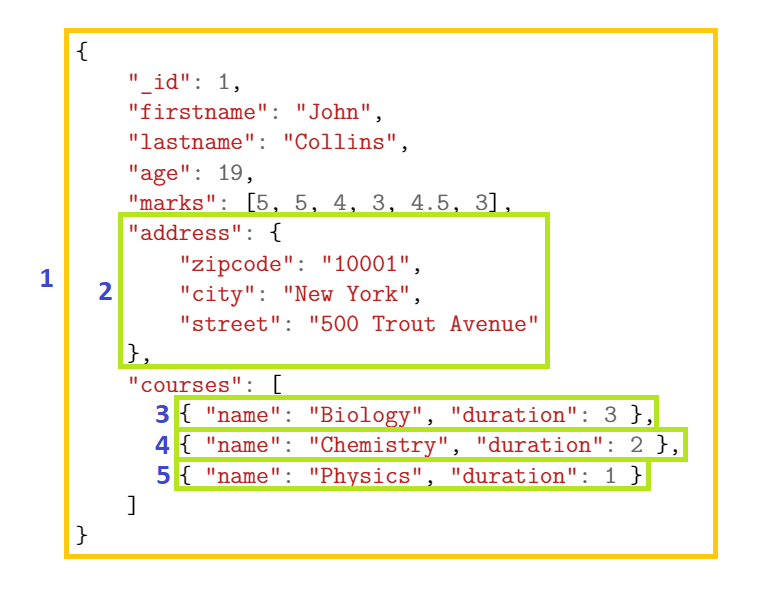
\includegraphics[width=12cm]{images/JSON-student.png}
\caption{Dokument z informacjami na temat studenta.}
\label{fig:dokument-student}
\end{figure}

\begin{figure}
\centering
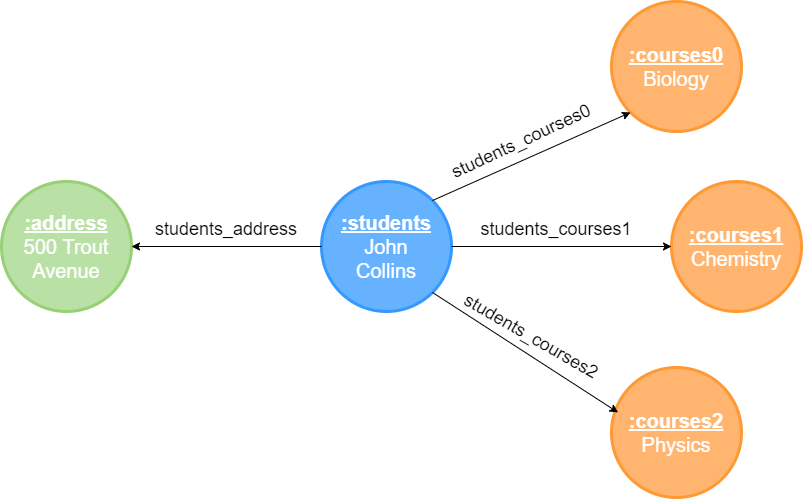
\includegraphics[width=12cm]{images/graf_student.png}
\caption{Odwzorowanie w grafie dokumentu opisującego studenta.}
\label{fig:graf-student}
\end{figure}

Na rysunku \ref{fig:dokument-student} żółtym prostokątem zaznaczono obiekt studenta, a zielonymi prostokątami wyróżniono obiekty zagnieżdżone. Wszystkie wyodrębnione obiekty oznaczono numerycznie. Każdy z zaznaczonych obiektów reprezentowany jest przez węzeł w~grafie wynikowym. Na rysunku \ref{fig:graf-student} można zaobserwować, że obiekt o numerze 1~przedstawiający studenta przekształcono w węzeł prezentowany kolorem niebieskim. Informacje o studencie, takie jak imię czy nazwisko, stały się właściwościami węzła. Etykieta węzła (\lstinline{students}) odpowiada nazwie kolekcji, w której znajdował się dokument. Dzięki temu, że obiekty zakorzenione w kolekcji odwzorowane są jako węzły z etykietami odpowiadającymi nazwie kolekcji, bez problemów wyszukać można grafy odpowiadające dokumentom wybranej kolekcji. 

Dokument adresu oznaczony numerem 2 został odwzorowany w grafie jako węzeł prezentowany kolorem zielonym, a informacje takie jak ulica lub miasto przekształcono we właściwości węzła. Zagnieżdżenie odwzorowano za pomocą krawędzi łączącej węzeł studenta z węzłem adresu. Etykieta węzła adresu odpowiada nazwie pola przechowującego zagnieżdżony dokument. Etykieta krawędzi powstała poprzez złączenie etykiet węzłów adresu i studenta. 

Listę liczb oznaczających oceny odwzorowano w grafie jako właściwość węzła studenta. Lista kursów składa się z obiektów oznaczonych numerami 3, 4 i 5. Każdy z tych obiektów przekształcono w węzeł prezentowany na grafie kolorem pomarańczowym. Informacje o nazwie i czasie trwania kursu stały się właściwościami węzła. Etykieta obiektu będącego elementem listy stanowi nazwę pola, zawierającego tę listę z dołączoną na końcu liczbą oznaczającą pozycję elementu w liście. Węzły kursów połączono krawędziami z węzłem studenta. Etykiety krawędzi powstały poprzez złączenie etykiet węzłów kursów i studenta.

Przy przekształcaniu kolekcji dokumentów w strukturę grafu warto rozważyć sposób odwzorowania listy elementów typu prostego. Głównym wyznacznikiem są możliwości systemu grafowego - jeśli system pozwala na przechowywanie list jako właściwości węzła, to warto skorzystać z takiej opcji. W sytuacji gdy system grafowy nie daje takiej możliwości, można przedstawić każdy z elementów listy jako osobny węzeł połączony krawędzią z węzłem dokumentu zawierającego listę. Etykieta węzła i krawędzi tworzona byłaby na takiej samej zasadzie, jak w przypadku listy dokumentów złożonych.

W rzadkich przypadkach, relacje pomiędzy dokumentami mogą być realizowane poprzez przechowywanie identyfikatorów dokumentów. Problematyczne w~tym przypadku jest rozróżnienie, czy dane pole dokumentu jest referencją do innego dokumentu czy nie. Niektóre magazyny dokumentów pozwalają na przechowywanie identyfikatorów w formie zmiennej referencyjnej. Pracując z takim systemem można sprawdzać, czy wartość danego pola jest referencją i wyszukiwać odpowiadający jej dokument, w celu odwzorowania relacji w grafie w postaci krawędzi. W proponowanym sposobie replikacji nie uwzględniono rozróżniania, czy pole jest referencją bądź listą referencji, a pola tego rodzaju traktowane są standardowo, jak pozostałe pola opisujące obiekt.

Przedstawione reguły replikacji danych między bazą dokumentową a grafową są regułami uniwersalnymi i pozwalają odwzorować dowolną kolekcję w postaci etykietowanych grafów skierowanych. Różne systemy bazodanowe zapewniają zróżnicowane funkcje i Interfejsy Programowania Aplikacji (ang. \ang{API - Application Programming Interface}), od których zależy łatwość zaimplementowania reguł replikacji, lecz powinny się one sprawdzić w~każdej implementacji bazy.

\chapter{Przegląd istniejących narzędzi replikacji}

W rozdziale dokonano przeglądu narzędzi wspierających replikację i zdecydowano się skoncentrować rozważania na narzędziach dla baz MongoDB i Neo4j, ponieważ dla tych implementacji udało się znaleźć największą liczbę rozwiązań. Przeprowadzono analizę dostępnych dla tych baz narzędzi oraz mechanizmów wspierających replikację. Należy pamiętać, że potrzeba replikacji danych pomiędzy SZBD o różnych modelach jest stosunkowo niszowa, przez co ograniczona jest liczba dostępnych publicznie narzędzi wspierających taki proces.

Przedstawione są dwa rozwiązania oparte o Mongo Connector, czyli Neo4j Doc Manager i Doc2graph, a także alternatywne rozwiązanie w postaci Mongo4j, które jest wtyczką do biblioteki modelowania obiektowego Mongoose. Przedstawiono także dwa zestawy mechanizmów, które mogą posłużyć do implementacji nowych narzędzi, czyli Change Streams dostępne w nowszych wersjach MongoDB, oraz Neo4j Streams, które może posłużyć do realizacji procesu replikacji w przeciwną stronę, czyli z bazy grafowej do dokumentowej.

\vspace{3.2cm}

\section{Podstawy techniczne} 

Implementacja replikacji pomiędzy bazą dokumentową a grafową jest zależna od mechanizmów dostępnych w rozpatrywanych bazach. MongoDB i Neo4j nie wspierają żadnego sposobu bezpośredniego połączenia systemów, więc konieczne jest wykorzystanie narzędzi zewnętrznych. Zadaniem takich narzędzi jest wykrywanie zmian w jednej bazie, konwersja danych do modelu grafowego i wstawianie ich do bazy docelowej. W takiej sytuacji szczególnie istotny jest system źródłowy, który musi umożliwiać wydajne wykrywanie i odczytywanie wprowadzanych zmian.

MongoDB posiada mechanizm dziennika operacji (ang. \ang{oplog - operations log}), w którym zapisywane są wszystkie operacje, które w jakikolwiek sposób modyfikują stan danych. Dziennik aktywny jest tylko w systemach skonfigurowanych do korzystania z zestawu replik (ang. \ang{replica set}), choć wystarczające jest wykorzystanie tylko jednej instancji repliki. Każdy wpis w dzienniku zawiera dokładny znacznik czasowy, rodzaj operacji, identyfikator obiektu na którym wykonano zmianę i~wszelkie istotne parametry. Kopia dziennika operacji dostępna jest dla użytkownika w postaci kolekcji \lstinline{local.oplog.rs}.

Dziennik operacji zapewnia łatwy sposób na śledzenie zmian w bazie dokumentowej. Na tym mechanizmie oparte jest rozwiązanie Mongo Connector, które śledzi zmiany w kolekcji dziennika i reaguje na nie wykonując adekwatne operacje w bazie docelowej. Takie rozwiązanie jest bardzo wydajne, dużo lepsze niż na przykład regularne odpytywanie (ang. \ang{polling}) bazy i porównywanie ze stanem poprzednim.

Kwestia wprowadzania danych do docelowej bazy Neo4j jest mniej problematyczna. Do wprowadzania zmian w bazie grafowej wystarczający jest dowolny interfejs, który pozwala na wykonywania poleceń Cypher. Może to być na przykład narzędzie konsolowe Cypher Shell lub dowolny sterownik pozwalający na połączenie z bazą z kodu aplikacji - dostępne są m.in. sterowniki dla Javy, Pythona, Go i~wielu innych języków \cite{bib:neo4j-drivers}.

Niezależnie od sposobu odczytywania i wprowadzania zmian w obu bazach, narzędzie musi obsługiwać konwersję pomiędzy modelem dokumentowym a grafowym. Bardzo ważne jest odpowiednie tworzenie węzłów i relacji dla dokumentów zagnieżdżonych i list, tak by przenieść maksymalnie dużo informacji z jednego systemu do drugiego. Dodatkową trudnością może być odpowiednia obsługa edycji - przed wstawieniem nowych danych narzędzie musi sprawdzić stan bazy i odpowiednio zedytować lub usunąć istniejące obiekty.  

\section{Mongo Connector}

Mongo Connector \cite{bib:mongo-connector-github, bib:mongo-connector-introducing} to generyczne narzędzie napisane w języku Python, pozwalajace na integrację MongoDB z dowolnym systemem zewnętrznym. Przy starcie narzędzia, kopiuje ono wszystkie obecnie istniejące dokumenty do systemu docelowego, a następnie monitoruje i dynamicznie przenosi kolejne zmiany. Jeśli Mongo Connector zostanie zatrzymany, możliwe jest wznowienie procesu replikacji od ostatniego działania, dzięki czemu zachowana jest spójność systemów.

Implementacja Mongo Connector'a oparta jest o dziennik operacji (oplog) dostępny w MongoDB po uruchomieniu zestawu replik (ang. \ang{replica set}). Specjalny wątek \textit{OplogThread} obsługuje aktywny kursor do kolekcji dziennika zdarzeń i wykrywa wszystkie nowe wpisy. Jeśli wpis dotyczy operacji zmieniającej stan danych, wywoływana jest odpowiednia funkcja zwrotna (ang. \ang{callback}), która określa czy dokonano wstawienia, edycji czy usuwania danych.

Integracja z dowolnym systemem docelowym realizowana jest za pomocą interfejsu \textit{DocManager} \cite{bib:mongo-connector-doc-manager}, który użytkownik może zaimplementować według własnych potrzeb. Każdy menedżer musi implementować klasę bazową \textit{DocManagerBase}, w~której zawarte są funkcje zwrotne wywoływane w reakcji na zmiany w bazie MongoDB. Twórcy Mongo Connector'a udostępniają kilka gotowych menedżerów, w tym dla systemów Elasticsearch oraz Solr. Oprócz tego, można znaleźć implementacje \textit{DocManager'a} innych autorów, które wstawiają dane do bazy Neo4j - dwa z takich rozwiązań zostaną przedstawione w kolejnych podsekcjach.

Mongo Connector jest narzędziem w pełni otwartym, a jego kod dostępny jest w repozytorium GituHub \cite{bib:mongo-connector-github}. Główną wadą narzędzia jest jego nieaktualność - ostatnie aktualizacje były wprowadzane w 2018 roku. Implementacja nie jest dostosowana do nowszych wersji MongoDB - najnowsza kompatybilna wersja bazy to MongoDB 3.6, które nie jest już oficjalnie wspierane.

\vspace{0.6cm}

\subsection{Neo4j Doc Manager}

Neo4j Doc Manager \cite{bib:neo4j-doc-manager-github} to implementacja interfejsu \textit{DocManager} Mongo Connector'a stworzona przez firmę Neo4j. Zadaniem narzędzia jest jednostronna synchronizacja danych pomiędzy bazą dokumentową MongoDB a bazą grafową Neo4j. Rozwiązanie reklamuje się obsługą wszystkich standarowych operacji na danych dostępnych w MongoDB. Wspierane są także złożone dokumenty o dowolnej strukturze. Zaprojektowane przez twórców zasady konwersji obejmują wszystkie informacje przechowywane w MongoDB, tak aby replikacja była całkowicie bezstratna i potencjalnie odwracalna. 

Implementacja przygotowana jest w całości w języku Python, podobnie jak Mongo Connector, co pozwala bardzo łatwo zintegrować oba narzędzia. Wszystkie funkcje narzędzia są bardzo precyzyjnie udokumentowane na oficjalnej stronie Neo4j \cite{bib:neo4j-doc-manager}. Dostępne są również przykłady wykorzystania i testy integracyjne. 

Podobnie jak w przypadku Mongo Connector'a, narzędzie nie jest aktywnie aktualizowane, a ostatnie zmiany zostały wprowadzone w 2016 roku. Implementacja nie jest dostosowana do nowych wersji Neo4j i firma nie wspiera narzędzia, jednak kod źródłowy dostępny jest w publicznym repozytorium GitHub, dzięki czemu możliwa jest samodzielna aktualizacja implementacji.

\subsection{Doc2graph} 

Drugą wybraną implementacją interfejsu \textit{DocManager} jest narzędzie Doc2graph \cite{bib:doc2graph-github}. Rola narzędzia jest podobna do poprzedniego - jego celem jest dynamiczne przenoszenie danych do bazy grafowej, tak aby wykorzystać zalety modelu grafowego podczas analizy danych. Pierwotnym źródłem danych dla narzędzia była wielomodelowa baza Couchbase, dopiero w późniejszej fazie dodano wsparcie dla MongoDB. 

Doc2graph składa się z dwóch części - wtyczki (ang. \ang{plugin}) do bazy Neo4j napisanej w Javie i prostej implementacji interfejsu \textit{DocManager} napisanej w Pythonie. Wtyczka zawiera implementację dwóch procedur dodawanych do Neo4j: \lstinline{json.upsert} i \lstinline{json.delete}. Klasa \textit{DocManager}'a wywołuje odpowiednie procedury w reakcji na zmiany w bazie dokumentowej. Implementacja wtyczki do komunikacji z bazą Neo4j korzysta z oficjalnych sterowników dla języka Java \cite{bib:neo4j-drivers}.

Ciekawą cechą narzędzia jest możliwość konfiguracji pewnych elementów logiki konwersji dokumentów na model grafowy. Konfigurację realizuje się poprzez dodanie do bazy Neo4j węzła o odpowiednio nazwanych właściwościach. W przypadku braku takiego węzła, wykorzystywana jest domyślna konfiguracja. Możliwa jest konfiguracja następujących opcji:

\begin{itemize}
\item strategia tworzenia etykiet węzłów,
\item strategia tworzenia etykiet relacji,
\item strategia tworzenia identyfikatora węzłów,
\item nazwa właściwości przechowującej pole identyfikatora \lstinline{_id} z bazy MongoDB.
\end{itemize}

Dla pierwszych trzech opcji możliwe jest wskazanie jednej z kilku klas implementujących dany fragment logiki. 

Podstawową wadą narzędzia Doc2graph jest brak wsparcia dla wszystkich standardowych operacji dostępnych w MongoDB. Część interfejsu \textit{DocManager} pozostała niezaimplementowana, co znacznie ogranicza przydatność narzędzia. Nie zaimplementowano m.in operacji edycji - by zmodyfikować istniejący obiekt konieczne jest usunięcie i ponowne wstawienie dokumentu w bazie źródłowej. Podobnie jak poprzednie Neo4j Doc Manager, projekt Doc2graph nie jest aktywnie utrzymywany i nie ma planów na uzupełnienie implementacji.

\section{Mongo4j}

Narzędzie Mongo4j \cite{bib:mongo4j-npm, bib:mongo4j-github} przedstawia zupełnie inne, alternatywne podejście do procesu replikacji. Mongo4j jest wtyczką do biblioteki Mongoose \cite{bib:mongo4j-mongoose}, zajmującej się mapowaniem obiektowym (ang. \ang{ODM - Object Data Modeling}) w aplikacjach opartych o Node JS.

Samo narzędzie Mongoose to biblioteka, która stanowi obiektowy interfejs do pracy z MongoDB. Pozwala definiować modele danych w postaci schematów (ang. \ang{schema}) i operować na instancjach tych modeli. Instancje obiektów można zapisywać i odczytywać z bazy dokumentowej, korzystając z automatycznego mapowania, z zapewnieniem wszystkich zdefiniowanych walidacji. W ten sposób narzędzie pełni analogiczną rolę co narzędzia mapowania obiektowo-relacyjnego (ang. \ang{ORM - object-relational mapping}) stosowane dla baz relacyjnych. 

Wtyczka Mongo4j rozszerza działanie biblioteki Mongoose, o możliwość równoczesnego zapisu danych w bazie dokumentowej MongoDB i grafowej Neo4j. Celem Mongo4j jest zminimalizowanie zmian potrzebnych w kodzie, by uzyskać duplikację danych - większość implementacji pozostaje identyczna jak przy wykorzystaniu jedynie Mongoose. Dodatkowa konfiguracja jest minimalna i polega jedynie na skonfigurowaniu połączenia do bazy Neo4j i określeniu które schematy i pola mają być replikowane w bazie grafowej. Operowanie na danych w większości pozostaje bez zmian. Wykonanie metod zapisu z biblioteki Mongoose powoduje, że Mongo4j automatycznie wstawia dane do Neo4j. W przypadku operacji edycji i~usuwania, zamiast bezpośredniego wywołania metod Mongoose konieczne jest wywołanie metod opakowujących dostępnych w Mongo4j, lecz ich interfejs jest spójny z Mongoose, więc zamiana jest bardzo prosta.  

Mongo4j pełni inną rolę niż rozwiązania oparte o Mongo Connector. Wcześniejsze narzędzia opierają się na monitorowaniu zmian wprowadzanych w bazie dokumentowej, a Mongo4j jest częścią aplikacji korzystającej z bazy, nie zapewnia zatem replikacji danych wprowadzanych bezpośrednio do bazy, z pominięciem aplikacji. Dodatkowo jest mniej odporne na wszelkie problemy z dostępnością bazy grafowej - ponieważ nie korzysta z żadnego dziennika operacji, jeśli tymczasowo utracone zostanie połączenie z bazą docelową, to nie ma możliwości wznowienia replikacji po odzyskaniu połączenia.

Autor zaznacza, że motywacją do stworzenia rozwiązania był brak pełnej satysfakcji z istniejących rozwiązań takich jak np. opisany wcześniej Neo4j Doc Manager, który potrzebuje dodatkowej warstwy poza aplikacją do instalacji i uruchamiania. Mongo4j jest wciąż aktywnie utrzymywane i dostosowane jest do najnowszych wersji MongoDB, Neo4j oraz biblioteki Mongoose. W repozytorium dostępny jest także komplet testów jednostkowych, które pokrywają wszystkie podstawowe przypadki użycia narzędzia i jednocześnie pełnią rolę przystępnych przykładów wykorzystania narzędzia w praktyce.

\vspace{1.6cm}

\section{Change Streams}

Rozpatrując inne podejścia do realizacji replikacji, bardzo obiecującym mechanizmem dostępnym w MongoDB od wersji 3.6 są tzw. Change Streams \cite{bib:change-streams, bib:change-streams-manual}, czyli strumienie zmian. Realizują podobną funkcję co Mongo Connector - dostarczają informacji o modyfikacjach wprowadzanych w bazie MongoDB. Strumienie zmian są zintegrowane z bazą MongoDB i dostępne są za pomocą dowolnego sterownika do komunikacji z bazą lub bezpośrednio za pomocą narzędzia powłoki Mongo Shell. Podobnie jak dziennik operacji (oplog), strumienie zmian wymagają uruchomienia zestawu replik (ang. \ang{replica set}) z przynajmniej jedną instancją repliki. 

Strumienie zmian przesyłają informacje zbliżone do formatu dziennika operacji, z którego korzysta Mongo Connector. Dostarczane są informacje o rodzaju zmiany, powiązanym dokumencie i wszelkie istotne parametry wykonanej operacji. Strumienie są wysoce konfigurowalne, możliwe jest nasłuchiwanie na zmiany na poziomie dowolnej bazy lub pojedynczej kolekcji, a także filtrowanie wyników, tak by zgłaszane były tylko wydarzenia odpowiadające potrzebom użytkownika. 

Dodatkową zaletą Change Streams jest możliwość odtworzenia wszystkich zdarzeń od wybranego momentu w czasie. Każde zdarzenie zawiera unikalny identyfikator chwili czasu, który można podać przy tworzeniu nowego strumienia, by kontynuować nasłuchiwanie od dowolnego momentu. Takie rozwiązanie pozwala reagować na wszelkie awarie i w razie potrzeby powtarzać pewne działania.

Obecnie nie istnieją gotowe narzędzia, które wykorzystują strumienie zmian do replikacji danych z bazy MongoDB do bazy grafowej, jednak warto rozpatrzeć ten mechanizm jako możliwą podstawę do implementacji całkiem nowego rozwiązania, które byłoby bardziej wydajne i aktualne niż omawiane wcześniej narzędzia oparte o Mongo Connector.  

\section{Neo4j Streams}

Jako rozszerzenie podstawowego tematu pracy, czyli replikacji z bazy dokumentowej do bazy grafowej, sprawdzano także możliwość replikacji danych w przeciwną stronę, czyli z bazy grafowej do dokumentowej. Nie istnieją żadne publicznie dostępne gotowe rozwiązania, które realizują taką operację, jednak potencjalnie możliwe jest stworzenie takiego mechanizmu, w oparciu o wtyczkę Neo4j Streams i rozszerzenia APOC dostępne w bazie Neo4j.

Neo4j Streams \cite{bib:neo4j-streams-github, bib:neo4j-streams} umożliwia integrację bazy Neo4j z narzędziami do strumieniowania wiadomości, takimi jak Apache Kafka. Możliwe jest zarówno automatyczne wstawianie danych do bazy grafowej w wyniku otrzymywanych wiadomości, jak i wysyłanie wiadomości o wykonanych operacjach. Wykorzystując dodatkowo rozszerzenia z biblioteki APOC \cite{bib:neo4j-apoc}, które umożliwiają tworzenie dowolnych wyzwalaczy uruchamianych na skutek dowolnych operacji, możliwe jest informowanie o wszystkich modyfikacjach danych wykonywanych w bazie Neo4j. Odpowiednia implementacja narzędzia reagującego na takie informacje, konwertującego dane do postaci dokumentów i wstawiającego je do bazy docelowej, pozwoliłaby uzyskać efekt replikacji z bazy grafowej do dokumentowej. 

\section{Podsumowanie}

Mimo że replikacja danych pomiędzy bazą dokumentową a bazą grafową jest rzadko spotykana, istnieją gotowe narzędzia, które na celu mają wspieranie takiej operacji. Niestety, większość z nich to narzędzia przestarzałe i niedostosowane do nowszych wersji baz danych. Narzędzie Mongo Connector i oparte na nim Neo4j Doc Manager i Doc2graph w teorii najlepiej realizuje zagadnienie omawiane w~pracy, jednak jego użycie wymaga wykorzystania nieaktualnej wersji MongoDB, co jest niewskazane w nowych projektach. 

Jedynym aktualnym i aktywnie wspieranym narzędziem jest Mongo4j, jednak nie jest to niezależne narzędzie realizujące replikację, a jedynie wtyczka do biblioteki mapowania obiektowego Mongoose. To narzędzie nadaje się do użycia tylko w~przypadku aplikacji opartych o Node JS i wykorzystujących bibliotekę Mongoose do operacji na danych.

Oprócz przedstawionych narzędzi można znaleźć także inne, które nie zostały przedstawione, ponieważ są zbyt proste i ograniczone lub nie są dostatecznie udokumentowane. W szczególności dostępne jest kilka alternatyw dla Mongo4j, które również rozszerzają bibliotekę Mongoose. Są to m.in. Moneo \cite{bib:moneo} i Neomongoose \cite{bib:neomongoose}, jednak ich zakres funkcji jest mniej rozbudowany niż w przypadku Mongo4j.

Alternatywą dla istniejących narzędzi jest stworzenie całkiem nowego rozwiązania replikacji pomiędzy bazą dokumentową a grafową, które byłoby bardziej nowoczesne i wydajne. Projektując takie rozwiązanie, warto rozważyć wykorzystanie mechanizmów Change Streams i Neo4j Streams. Należy jednak pamiętać, że oba mechanizmy są wciąż aktywnie rozwijane i modyfikowane, co może skutkować koniecznością częstego aktualizowania rozwiązania wraz z kolejnymi wydaniami systemów MongoDB i Neo4j.

\chapter{Badania}

Dotychczas w pracy przybliżono tematykę dokumentowych i grafowych baz danych i opisano uniwersalne zasady replikacji danych pomiędzy takimi systemami. Przedstawiono również szczegółowo bazy MongoDB i Neo4j i wykonano analizę dostępnych mechanizmów i narzędzi, które umożliwiają proces replikacji pomiędzy tymi systemami. Badania przedstawione w tym rozdziale skupiają się na eksperymentach z wykorzystaniem trzech wybranych narzędzi: Neo4j Doc Manager, Doc2graph oraz Mongo4j. 

Celem badań jest przetestowanie wybranych narzędzi dla najpopularniejszych baz oraz ocena ich przydatności oraz zgodności z zaprezentowanym w pracy uniwersalnym zestawem reguł replikacji między bazą dokumentową a grafową. Sprawdzono, czy metody konwersji dokonywanej przez narzędzia pokrywają się z regułami i jakie występują różnice. Zweryfikowano jakie modyfikacje należałoby wprowadzić w narzędziach aby w większym stopniu pokrywały się z regułami. 

Ze względu na wymagania wynikające z konfiguracji i ograniczeń narzędzi, dla każdego z nich opracowano maksymalnie zbliżone do siebie schematy dokumentów. Podczas przedstawiania przypadków testowych, zaprezentowanych w podsekcjach \ref{section:struktury-proste}-\ref{section:rozbudowany-przykład}, dokładniej omówiono wykorzystane dokumenty i występujące między nimi różnice. Testowano działanie narzędzi w przypadku operacji dodawania, aktualizacji i usuwania danych w bazie dokumentowej. Pod koniec rozdziału dodatkowo oceniono stabilność narzędzi oraz kompletność przeprowadzanej przez nie replikacji.

\section{Przygotowanie narzędzi} 

Przed przystąpieniem do realizacji badań konieczne było przygotowanie wykorzystywanych w nich narzędzi. Każde narzędzie należało zainstalować wraz z wymaganymi zależnościami. Dodatkowo dwa z nich, Neo4j Doc Manager i Doc2graph, wymagały aktualizacji zależności oraz modyfikacji kodu źródłowego w celu dostosowania ich do pracy z aktualną wersją bazy Neo4j. W kolejnych podsekcjach omówiono proces przygotowania i uruchamiania każdego z narzędzi.

\subsection{Neo4j Doc Manager}

Narzędzie dostępne jest jako paczka w repozytorium Python Package Index (PyPI), więc w celu instalacji wystarczające jest wykonanie polecenia \texttt{pip install neo4j-doc-manager}. Niestety wersja narzędzia dostępna w repozytorium jest nieaktualna i próby jej uruchomienia skutkują błędami. W zależnościach narzędzia zdefiniowana jest biblioteka py2neo w wersji 2.0.8, która nie jest już publicznie dostępna. By wykorzystać Neo4j Doc Manager w badaniach konieczne było wprowadzenie modyfikacji w kodzie źródłowym narzędzia, by dostosować je do pracy z~najnowszą wersją biblioteki py2neo. Zmiany wdrożono w czterech plikach:

\begin{itemize}
\item \texttt{neo4j\_doc\_manager.py},
\item \texttt{nodes\_and\_relationships\_builder.py},
\item \texttt{nodes\_and\_relationships\_updater.py}, 
\item \texttt{error\_handler.py}.
\end{itemize}

Nieaktualne metody występujące w trzech pierwszych plikach zastąpiono ich odpowiednikami pochodzącymi z najnowszej implementacji biblioteki py2neo. Były one związane przede wszystkim z rozpoczynaniem transakcji w bazie grafowej i realizowanymi w ramach tej transakcji operacjami. Dodatkowo w drugim i trzecim pliku dostosowano sposób przekazywania parametrów do zapytań Cypher, tak by były zgodne ze składnią nowej wersji Neo4j. W trzecim pliku dostosowano odczytywanie dziennika zdarzeń, tak by obsłużyć dodatkowe pole określające wersję dokumentu, które pojawiło się w wersji 3.6 bazy MongoDB. 

Następną konieczną zmianą było dostosowanie pliku \lstinline{error_handler.py}, w~którym zdefiniowane są wszystkie błędy, które mogą wystąpić podczas operowania na bazie grafowej. Postanowiono zostawić wyłącznie obsługę generycznych błędów, ponieważ w najnowszej wersji biblioteki py2neo nie istnieje obsługa błędów w takiej postaci, jak w wersji 2.0.8. Możliwa jest implementacja bardziej precyzyjnej obsługi błędów, w której zwracane byłyby szczegółowe opisy pojawiających się błędów, jednak na potrzeby wykonania badań, generyczna obsługa błędów jest wystarczająca.

Przed wykonaniem komendy uruchamiającej narzędzie, konieczne jest zainicjowanie zestawu replik w MongoDB. W tym celu należy uruchomić MongoDB z odpowiednim przełącznikiem \texttt{--replSet}, a następnie w powłoce bazy wykonać polecenie \texttt{rs.initiate()}. Po przygotowaniu bazy i narzędzia, proces replikacji można zainicjować poprzez polecenie \texttt{mongo-connector}, przekazując w nim w~odpowiednich parametrach adresy baz MongoDB i Neo4j oraz przełącznik \texttt{-d neo4j\_doc\_manager}, wskazujący z której implementacji interfejsu \texttt{DocManager} należy skorzystać.

\subsection{Doc2graph}

Doc2Graph dostępne jest w repozytorium GitHub, skąd można pobrać kod źródłowy narzędzia. Część implementacji w jęzku Python również wykorzystuje bibliotekę py2neo, przez co konieczne są podobne zmiany co dla Neo4j Doc Manager. Poprawiono kod źródłowy w następujących plikach:

\begin{itemize}
\item \texttt{setup.py},
\item \texttt{neo4j\_json\_doc\_manager.py},
\item \texttt{error\_handler.py}.
\end{itemize}

Tutaj również w pliku \texttt{error\_handler.py} zredukowano obsługę błędów do błędów generycznych, a w pliku \texttt{neo4j\_json\_doc\_manager.py} zaktualizowano sposób rozpoczynania transakcji i wykonywania w ramach niej operacji. Dodatkowo edytowano plik \texttt{setup.py} w celu wymuszenia pobierania biblioteki py2neo w najnowszej dostępnej wersji. Mniejsza obszerność kodu w języku Python wynika z faktu, że większość logiki narzędzia Doc2graph zawarta jest we wtyczce do Neo4j o nazwie neo4j-json napisanej w języku Java.

W projekcie neo4j-json zmieniono wersję zależności sterowników dla Neo4j, tak by odpowiadała najnowszej wersji bazy i zaktualizowano część testów jednostkowych. Aktualizacja zależności spowodowała, że konieczne było wprowadzenie modyfikacji w kodzie m.in. wprowadzając obsługę transakcji. Po aktualizacji kodu, w ramach pojedynczej operacji wykonywana jest jedna transakcja, dzięki czemu w~przypadku awarii zmiany są wycofywane, zamiast zostać zrealizowane częściowo. 

Dodatkowo konieczna była zmiana w logice tworzenia etykiet krawędzi pomiędzy węzłami. Domyślna implementacja tworzy etykiety wykorzystując identyfikator dokumentu (pole \texttt{\_id}) węzła rodzica - takie rozwiązanie nie działa w~nowszych wersjach Neo4j, w których etykiety nie mogą rozpoczynać się od liczby. W~związku z tym, w procesie tworzenia etykiet krawędzi dodano dołączanie przedrostka ``KEY\_''.

\begin{lstlisting}[style=Cypher, caption={Konfiguracja Doc2graph.}, label={listing:konfiguracja-doc2graph}, captionpos=b]
CREATE (n:JSON_CONFIG {
  configuration: 'byNode',
  root_node_key_property: '_id',
  document_default_label: 'DocNode',
  document_id_builder: 'org.neo4j.helpers.json.
    document.impl.DocumentIdBuilderId',
  document_relation_builder: 'org.neo4j.helpers.json.
    document.impl.DocumentRelationBuilderByKey',
  document_label_builder: 'org.neo4j.helpers.json.
    document.impl.DocumentLabelBuilderById',
  log_discard_events: false
})
\end{lstlisting}

Wtyczka neo4j-json umożliwia skonfigurowanie m.in. sposobu tworzenia relacji, identyfikatorów węzłów oraz etykiet. Na potrzeby badań zdecydowano się na konfigurację przedstawioną na listingu \ref{listing:konfiguracja-doc2graph}. Przy takiej konfiguracji wymagane jest, aby wszystkie dokumenty zawierały pole \texttt{id}. Wykorzystanie domyślnej konfiguracji wymagałoby dodatkowo poza polem \texttt{id} dodania w dokumentach pola \texttt{type}. Konfigurację ustala się poprzez dodanie odpowiedniego węzła w bazie Neo4j, a~następnie zrestartowanie systemu. Na rysunku \ref{fig:węzeł-konfiguracji} przedstawiono węzeł przechowujący konfigurację z listingu \ref{listing:konfiguracja-doc2graph}.

\begin{figure}
\centering
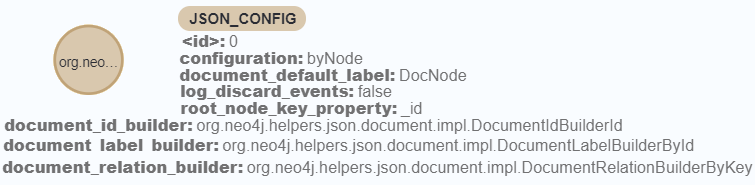
\includegraphics[width=12cm]{images/węzeł konfiguracji doc2graph.png}
\caption{Węzeł konfiguracji dla Doc2graph.}
\label{fig:węzeł-konfiguracji}
\end{figure}

Przed rozpoczęciem pracy z Doc2graph konieczna jest ręczna instalacja narzędzia Mongo Connector. Jest ono dostępne w repozytorium PyPI, a w celu jego instalacji wykonano polecenie \texttt{pip install mongo-connector}. Po przygotowaniu narzędzi wgrano skompilowaną wtyczkę neo4j-json do bazy Neo4j, dodano węzeł konfiguracyjny i zrestartowano system. Przekazanie danych uwierzytelniania do baz oraz uruchomienie procesu replikacji dokonuje się w taki sam sposób, jak w~przypadku narzędzia Neo4j Doc Manager.

\subsection{Mongo4j}

Mongo4j jest wtyczką do biblioteki Mongoose służącej do modelowania obiektów w bazie MongoDB. Mongoose wykorzystywane jest w aplikacjach uruchamianych w środowisku Node JS. W przeciwieństwie do poprzednich dwóch narzędzi, Mongo4j jest aktywnie wspierany. Podczas badań wykorzystano wersję 4.0.1 z września 2021 roku oraz Mongoose w najnowszej dostępnej wersji. 

Ponieważ Mongoose jest narzędziem mapowania obiektowego, konieczne jest utworzenie modeli obiektów, czyli tzw. schematów (ang. \ang{Schema}). Definiuje się je w kodzie JavaScript. Przykład prostego schematu dla obiektów typu \lstinline{Student} przedstawiono na listingu \ref{listing:Schemat-student}. Na potrzeby badań, w analogiczny sposób przygotowano schematy wszystkich obiektów wykorzystywanych w przypadkach testowych. W każdym z opracowanych schematów, dla każdego pola ustawiono wartość zmiennej \texttt{neo\_prop} jako ``true'', dzięki czemu pola objęte są replikacją do bazy grafowej.

Instalacja narzędzia Mongo4j jest bardzo prosta i szybka. W pierwszej kolejności zainstalowano Node JS. Następnie konieczne było pobranie i instalacja biblioteki Mongoose poprzez polecenie \texttt{npm install mongoose --save}. Na końcu zainstalowano Mongo4j wykonując komendę \texttt{npm install --save mongo4j}. Kod wykorzystywany podczas badań zawarto w plikach napisanych w JavaScript. Zaimportowano w nich Mongoose oraz Mongo4j, a następnie skonfigurowano nawiązanie połączenia z bazą Neo4j oraz MongoDB. Wszystkie operacje na przygotowanych schematach zaimplementowane są w tych plikach. Mając tak przygotowane narzędzia można w łatwy sposób przeprowadzić replikację wykonując przygotowany kod JavaScript za pomocą komendy \texttt{node plik.js}. 

\begin{lstlisting}[style=JS, caption={Przykładowy schemat dla obiektów typu Student.}, label={listing:Schemat-student}, captionpos=b]
const StudentSchema = new Schema({
    name: {
        type: String,
        neo_prop: true
    },
    age: {
        type: Number,
        neo_prop: true
    },
    score: {
        type: mongoose.Types.Decimal128,
        neo_prop: true
    },
    pass: {
        type: Boolean,
        neo_prop: true
    }
});
\end{lstlisting}

\section{Środowisko badań} 

Środowisko badań przygotowano korzystając z narzędzia Docker, czyli systemu operacyjnego dla kontenerów. Pozwala tworzyć kontenery bazując na przygotowanych wcześniej obrazach, zapewniając przenośność aplikacji. Umożliwia łatwe uruchomienie wybranej aplikacji na dowolnym systemie bez konieczności lokalnej instalacji wymaganych zależności i oprogramowania. Kontenery są konfigurowalne i~zawierają wszystkie narzędzia, zmienne środowiskowe i oprogramowania wymagane do działania aplikacji. Dzięki konteneryzacji, poszczególne systemy uruchamiane są jako niezależne serwisy komunikujące się za pomocą odpowiednich kanałów. 

Podczas pracy z kontenerami bardzo przydatnym narzędziem jest Docker Compose. Pozwala uruchamiać wiele kontenerów jednocześnie, wprowadzając przygotowaną dla nich konfigurację. W tym celu, dla danego zestawu kontenerów tworzy się plik konfiguracyjny docker-compose.yml. Przykładowy plik tego formatu wykorzystany podczas przeprowadzenia badań umieszczono w listingu \ref{listing:docker-compose-neo4jdocmanager}. Zawiera on konfigurację dla narzędzia Neo4j Doc Manager wraz z bazami Neo4j i MongoDB. Posiadając dedykowany plik konfiguracyjny, można bardzo szybko i łatwo uruchomić potrzebne serwisy wykonując komendę \texttt{docker-compose up} w lokacji pliku Docker Compose.

\begin{lstlisting}[style=JS, caption={Plik konfiguracyjny dla narzędzia Neo4j Doc Manager.}, label={listing:docker-compose-neo4jdocmanager}, captionpos=b]
version: "3.8"
services:
    neo4j:
        image: neo4j:4.3.3
        container_name: neo4j_neo4jdocmanager
        environment:
            NEO4J_AUTH: neo4j/admin
            NEO4JLABS_PLUGINS: '["apoc"]'
        ports:
            - 7474:7474
            - 7687:7687
        volumes:
            - neo4j_data_volume:/data
            
    mongo:
        image: mongo:3.6
        container_name: mongo_neo4jdocmanager
        environment:
            MONGO_INITDB_ROOT_USERNAME: admin
            MONGO_INITDB_ROOT_PASSWORD: admin
        ports:
            - 27017:27017      
        volumes:
            - mongo_data_volume:/data/db
        command: mongod --replSet rs0 
        healthcheck:
            test: test $$(echo "rs.initiate().ok 
            || rs.status().ok" | mongo -u admin 
            -p admin --quiet) -eq 1
        
    neo4j-doc-manager:
        image: oladyr/neo4j-doc-manager:1.0.0
        container_name: neo4j-doc-manager
        environment:
            NEO4J_AUTH: neo4j:admin
        tty: true

volumes:
    neo4j_data_volume:
    mongo_data_volume:
\end{lstlisting}

Na potrzeby badań skorzystano z oficjalnych obrazów udostępnionych dla baz Neo4j oraz MongoDB, które dostępne są w repozytorium Docker Hub \cite{bib:dockerhub-mongo, bib:dockerhub-neo}. Wykorzystane w badaniach obrazy zawierają Neo4j w wersji 4.3.3 oraz MongoDB w~wersji 3.6. Podczas wprowadzania koniecznych zmian w narzędziach dostosowano je do pracy z nową wersją Neo4j. W przypadku MongoDB, dostosowanie Mongo Connectora okazało się dużo trudniejsze, dlatego wykorzystano starszą wersję bazy zalecaną dla tego narzędzia.

Dla każdego z badanych narzędzi stworzono własny obraz z zainstalowanym narzędziem i wszystkimi potrzebnymi zależnościami. Następnie przygotowano pliki konfiguracyjne Docker Compose pozwalające na szybkie uruchomienie wybranego narzędzia wraz z bazami. Na listingu \ref{listing:docker-compose-neo4jdocmanager} dla narzędzia Neo4j Doc Manager zawarta jest konfiguracja woluminów, która pozwala trwale zachować stan każdej z~baz. Dodatkowo określone są zmienne środowiskowe przechowujące dane uwierzytelniania. Zdefiniowano również mapowanie portów między kontenerem a lokalnym systemem. Podczas badań kontenery dla każdego narzędzia uruchamiano osobno, tak aby narzędzia nie wpływały na siebie wzajemnie.  

W trakcie badań przeprowadzanych dla narzędzi Doc2graph i Neo4j Doc Manager do operowania na dokumentach skorzystano z aplikacji Robo 3T \cite{bib:robo3t}, która zapewnia interfejs dostępu do danych. W przypadku Mongo4j nie było takiej potrzeby, ponieważ dokumenty wstawiane są z poziomu kodu aplikacji. Efekty replikacji zrealizowanej w bazie grafowej obserwowano za pomocą graficznego interfejsu dostępnego z poziomu przeglądarki, który jest domyślnie dostępny dla bazy Neo4j. 

\section{Proces replikacji} 

W ramach przeprowadzanych badań, dla każdego wybranego narzędzia wykonano operacje wstawiania, edytowania oraz usuwania dokumentów. Działania te zrealizowano zarówno dla struktur prostych jak i złożonych. W kolejnych podsekcjach przedstawiono przebieg i efekty realizacji operacji na danych dla poszczególnych badanych przypadków. Testując kolejne narzędzia wykorzystano takie same struktury dokumentów, za wyjątkiem narzędzia Doc2graph, dla którego konieczne było dodanie we wszystkich dokumentach (w tym również zagnieżdżonych) pola \texttt{id}, wymaganego m.in. do tworzenia etykiet. 

Przed przejściem do przypadków testowych, omówione są podstawowe typy danych występujące w systemach MongoDB i Neo4j oraz sposób ich obsługi przez analizowane narzędzia.

\subsection{Wspierane typy danych}
\label{section:wspierane-typy-danych}

Baza dokumentowa MongoDB wspiera wiele różnych typów danych, spośród których tylko część wspierana jest przez analizowane narzędzia. Oprócz tego, MongoDB i Neo4j posiadają różne typy odpowiadające podobnym rodzajom danych i~niektórych typów nie da się jednoznacznie odwzorować w obu systemach, przez co narzędzia różnią się sposobem doboru docelowego typu danych.

W przypadku numerycznych typów danych, MongoDB wyróżnia cztery rodzaje: Double (alias ``double''), Decimal128 (``decimal''), 32-bit integer (``int'') oraz 64-bit integer (``long''). Neo4j posiada natomiast typ abstrakcyjny Number, dla którego istnieją podtypy Integer i Float. Wśród standardowych typów dla obu baz występują typy String oraz Boolean, które dla każdego narzędzia są analogicznie odwzorowywane.

Dla narzędzia Neo4j Doc Manager, typ Decimal128 konwertowany jest na String, Double na Float, a 64-bit integer oraz 32-bit integer na Integer. W przypadku typu Decimal128 taki sposób konwersji związany jest z koniecznością przechowywania określonej precyzji danej liczby. Gdyby został on przekształcony w~typ Float, zapisana liczba utraciłaby dokładną precyzję zapisu. Dzięki temu, że jest ona zapisana jako String, dokładność zapisu danej liczbowej jest zachowana co ma duże znaczenie na przykład w zastosowaniach bankowych i finansowych. Dla narzędzia Doc2graph konwersja typów przebiega niemal tak samo, z wyjątkiem typu Decimal128, który jest całkowicie pomijany przy odwzorowywaniu właściwości w~węźle. Mongo4j natomiast standardowo pozwala sprecyzować tylko dwa typy numeryczne: Number i Decimal128. Podczas wstawiania tego typu danych do węzła, zostają one skonwertowane odpowiednio na Integer oraz Float. Możliwość sprecyzowania innych typów numerycznych dostępna jest wyłącznie po zainstalowaniu dodatkowych wtyczek dla tego narzędzia.

Bardzo powszechną potrzebą jest stosowanie tablic (ang. \ang{array}) typów prostych. Zarówno Neo4j Doc Manager jak i Doc2graph obsługują typ tablicowy. Podczas odwzorowywania tego typu w bazie grafowej, jest on przekształcany w~listę wartości typu prostego. Mongo4j natomiast nie wspiera tablic i są one pomijane podczas replikacji. Dodatkowo żadne z badanych narzędzi nie obsługuje typu binarnego, a jego wykorzystanie powoduje wystąpienie błędu.

W przypadku typów określających czas, MongoDB wyróżnia typ Date i Timestamp a Neo4j wyróżnia typy Date, Time, LocalTime, DateTime, LocalDateTime oraz Duration. Dla narzędzia Neo4j Doc Manager typy Date oraz Timestamp konwertowane są na String. Doc2graph identycznie postępuje z typem Date ale typ Timestamp pomija przy replikacji. Mongo4j konwertuje Date na Integer, a innych typów standardowo nie obsługuje.   

W dokumentach możliwe jest stosowanie zagnieżdżonych dokumentów lub tablic zawierających dokumenty, co pozwala osiągnąć rozbudowane i skomplikowane struktury obiektów. Kwestia wspierania takich struktur przez narzędzia omawiana jest w kolejnych sekcjach podczas omawiania kolejnych przypadków testowych, ponieważ obsługa pól przechowujących dokumenty jest różna w zależności od wykonywanej operacji.

\subsection{Struktury proste}
\label{section:struktury-proste}

Pierwszy przypadek testowy sprawdza replikację prostego dokumentu niezawierającego obiektów zagnieżdżonych. Na listingu \ref{listing:json-struktura-prosta} zaprezentowano prostą strukturę dokumentu reprezentującego studenta. Dokument składa się z pola typu String przechowującego imię oraz pola tego samego typu przechowującego datę urodzenia, pola typu Integer z informacją o wieku, pola typu Double/Decimal związanego z wynikiem końcowym ze studiów oraz pola typu Boolean będącego flagą informującą czy student zaliczył wszystkie przedmioty.

\begin{lstlisting}[style=JSON, caption={Struktura prostego dokumentu.}, label={listing:json-struktura-prosta}, captionpos=b] 
{
  "name": "Adam",
  "age": 23,
  "dateOfBirth": "1998-02-03",
  "score": 99.8,
  "pass": true
}
\end{lstlisting}

Dokument z listingu \ref{listing:json-struktura-prosta} wstawiono do bazy MongoDB dla narzędzia Neo4j Doc Manager. Dla Mongo4j przygotowano schemat odpowiadający takiej samej strukturze. Na listingu \ref{listing:json-struktura-prosta-doc2graph} znajduje się analogiczna struktura rozszerzona o pole \texttt{id} utworzona dla narzędzia Doc2graph.



\begin{lstlisting}[style=JSON, caption={Struktura prostego dokumentu dla Doc2graph.}, label={listing:json-struktura-prosta-doc2graph}, captionpos=b]
{
  "id": 1,
  "name": "Adam",
  "age": 23,
  "dateOfBirth": "1998-02-03",
  "score": 99.8,
  "pass": true
}
\end{lstlisting}

Rezultatem replikacji dokumentu z wykorzystaniem Neo4j Doc Manager jest węzeł przedstawiony na rysunku \ref{fig:graf-struktura-prosta-neo4jdocmanager}. Utworzony węzeł posiada takie same właściwości i~wartości jak pola oryginalnego dokumentu, rozszerzone o właściwość \texttt{\_ts} przechowującą znacznik czasu utworzenia obiektu w bazie dokumentowej. Ponadto węzeł posiada dwie etykiety: \texttt{Document} informującą, że węzeł jest repliką struktury dokumentowej oraz \texttt{students}, która jest nazwą kolekcji dokumentów. 

\begin{figure}[!h]
\centering
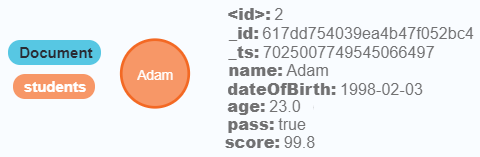
\includegraphics[width=12cm]{images/struktura_prosta_neo4jdocmanager.png}
\caption{Rezultat replikacji prostej struktury przez Neo4j Doc Manager.}
\label{fig:graf-struktura-prosta-neo4jdocmanager}
\end{figure}

Następnie ten sam dokument poddano edycji, zmieniając wartość pól \texttt{name} oraz \texttt{score}. Replikacja aktualizacji przebiegła pomyślnie i w węźle docelowym znalazły się nowe wartości dla zmodyfikowanych pól. Ostatnim testem dla Neo4j Doc Manager było usunięcie dokumentu z bazy dokumentowej, co również zostało poprawnie i natychmiastowo odwzorowane w Neo4j. 

Dla narzędzia Doc2graph w wyniku dodania struktury z listingu \ref{listing:json-struktura-prosta-doc2graph} otrzymano w bazie grafowej zreplikowany węzeł przedstawiony na rysunku \ref{fig:graf-struktura-prosta-doc2graph}. Węzeł posiada dokładnie takie same właściwości jak pola oryginalnego dokumentu. Dodatkowo nadana została mu etykieta \texttt{ID\_1} utworzona na podstawie pola \texttt{id}. 

\begin{figure}[!h]
\centering
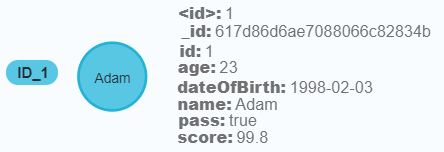
\includegraphics[width=12cm]{images/struktura_prosta_doc2graph.png}
\caption{Rezultat replikacji prostej struktury przez Doc2graph.}
\label{fig:graf-struktura-prosta-doc2graph}
\end{figure}

W przypadku Doc2graph próba edycji struktury dokumentowej skutkowała brakiem replikacji zmian w bazie grafowej - twórcy narzędzia nie zaimplementowali obsługi dla operacji edycji dokumentów. Narzędzie obsługuje wyłącznie operacje wstawiania i usuwania. Tak jak dla poprzedniego narzędzia, usunięcie struktury dokumentowej z bazy źródłowej zostało poprawnie odwzorowane w bazie grafowej. 

Na listingu \ref{listing:dokument-struktura-prosta-mongo4j} przedstawiono strukturę dokumentową dodaną do bazy MongoDB dla narzędzia Mongo4j w oparciu o przygotowany wcześniej schemat. Na rysunku \ref{fig:graf-struktura-prosta-mongo4j} umieszczono wynik odwzorowania dokumentu w bazie grafowej. 
\begin{figure}
\begin{lstlisting}[style=JSON, caption={Struktura prostego dokumentu wstawiona przez Mongo4j.}, label={listing:dokument-struktura-prosta-mongo4j}, captionpos=b]
{
  "_id" : ObjectId("617dac1deee6a319f221dd40"),
  "name" : "Adam",
  "age" : 23,
  "dateOfBirth" : "1998-02-03",
  "score" : NumberDecimal("99.8"),
  "pass" : true,
  "__v" : 0
}
\end{lstlisting}
\end{figure}
Można zaobserwować zmianę notacji dla pola daty urodzenia, z nazwy \texttt{dateOfBirth} na \texttt{date\_of\_birth}. Pole \texttt{\_id} struktury dokumentowej zostało odwzorowane jako właściwość \texttt{m\_id}. Wynikowy węzeł otrzymał etykietę \texttt{Student} stanowiącą nazwę modelu zbudowanego w oparciu o schemat.

\begin{figure}[!h]
\centering
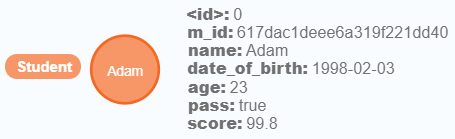
\includegraphics[width=12cm]{images/struktura_prosta_mongo4j.png}
\caption{Rezultat replikacji prostej struktury przez Mongo4j.}
\label{fig:graf-struktura-prosta-mongo4j}
\end{figure}

Następnie dokonano edycji obiektu poprzez modyfikację wartości pól \texttt{score} oraz \texttt{name}. Zarówno w strukturze dokumentowej w bazie MongoDB jak i w bazie grafowej aktualizacja została wprowadzona prawidłowo. Na końcu wykonano operację usunięcia obiektu, która również zakończyła się pomyślnie, skutkując usunięciem danych w obu bazach. 

\subsection{Obiekty zagnieżdżone}

Drugi rozpatrywany przypadek testowy sprawdza działanie replikacji w przypadku dokumentu zawierającego dokument zagnieżdżony. Rozpatrywana struktura przedstawiona jest na listingu \ref{listing:json-zagnieżdżenie}. Zawiera ona takie same pola jak omówiona wcześniej struktura prosta oraz jedno dodatkowe pole, przechowujące dokument zagnieżdżony adresu, który składa się z trzech pól typu String.

Strukturę z dokumentem zagnieżdżonym wstawiono do bazy dokumentowej przy włączonej replikacji narzędzia Neo4j Doc Manager. Otrzymany rezultat replikacji przedstawia rysunek \ref{fig:graf-struktura-zagnieżdżenie-neo4jdocmanager}. W Neo4j utworzone zostały dwa węzły: jeden odpowiadający obiektowi studenta a drugi obiektowi adresu. Węzeł reprezentujący studenta zawiera takie same właściwości jak węzeł uzyskany dla struktury prostej w poprzedniej podsekcji. Węzeł adresu posiada właściwości odpowiadające polom zagnieżdżonego dokumentu adresu i dodatkowo zawiera właściwości \texttt{\_ts} i~\texttt{\_id} o tych samych wartościach co węzeł studenta. 

\begin{lstlisting}[style=JSON, caption={Struktura dokumentu z obiektem zagnieżdżonym.}, label={listing:json-zagnieżdżenie}, captionpos=b]
{
  "name": "Adam",
  "age": 23,
  "dateOfBirth": "1998-02-03",
  "score": 99.8,
  "pass": true,
  "address": {
    "street": "500 Trout Avenue",
    "city": "New York",
    "zipCode": "10001"
  }
}
\end{lstlisting}

\begin{figure}[!h]
\centering
\captionsetup{justification=centering}
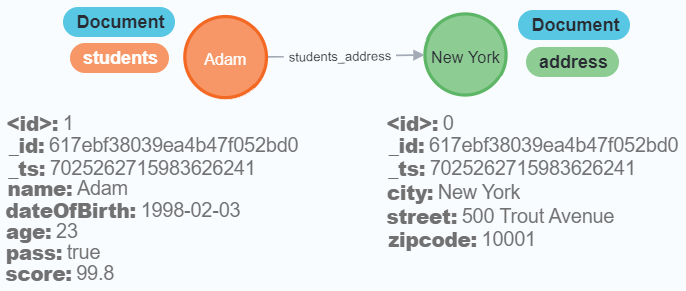
\includegraphics[width=12cm]{images/zagnieżdżenie_neo4jdocmanager.png}
\caption{Rezultat replikacji struktury z obiektem zagnieżdżonym przez Neo4j Doc Manager.}
\label{fig:graf-struktura-zagnieżdżenie-neo4jdocmanager}
\end{figure}

Obu węzłom przypisano etykietę \texttt{Document}, informującą o wykonanej replikacji z bazy dokumentowej. Oprócz tego, węzeł studenta posiada etykietę \texttt{students} odpowiadającą nazwie kolekcji dokumentów, a węzeł adresu posiada etykietę \texttt{address}, która została nadana na podstawie nazwy pola przechowującego obiekt adresu w~dokumencie źródłowym. Pomiędzy węzłami została utworzona krawędź skierowana w stronę węzła adresu, o etykiecie \texttt{students\_address}, której nazwa odpowiada nazwom etykiet powiązanych węzłów.

Następnie dokument poddano edycji poprzez modyfikację pól \texttt{score} oraz \texttt{city}. Neo4j Doc Manager nie wspiera bezpośredniego nadpisywania zagnieżdżonych obiektów - w celu edycji konieczne jest usunięcie pola przechowującego adres, a~następnie dodanie go w nowej formie ze zmienioną wartością pola \texttt{city}. Replikacja tak przeprowadzonych zmian przebiegła pomyślnie i odpowiednie właściwości zostały zmienione w węzłach. Co ciekawe, po wykonanej operacji z węzła adresu zniknęła właściwość \texttt{\_ts}. Na końcu z bazy dokumentowej usunięto strukturę studenta, w wyniku czego oba węzły zostały usunięte w bazie grafowej.

Przeprowadzenie testów dla Doc2graph wymagało dostosowania struktury dokumentu do postaci przedstawionej na listingu \ref{listing:json-zagnieżdżenie-doc2graph}, poprzez dodanie pól \texttt{id} do dokumentu studenta i zagnieżdżonego dokumentu adresu. W wyniku wstawienia struktury do bazy dokumentowej, na skutek replikacji za pomocą narzędzia Doc2graph otrzymano rezultat przedstawiony na rysunku \ref{fig:graf-struktura-zagnieżdżenie-doc2graph}. Tutaj również powstały dwa węzły, jeden dla studenta i jeden dla adresu, połączone krawędzią skierowaną do obiektu adresu. Wszystkie pola struktury dokumentowej zostały odwzorowane poprawnie zarówno dla studenta jak i adresu. 

\begin{lstlisting}[style=JSON, caption={Struktura dokumentu z obiektem zagnieżdżonym dla Doc2graph.}, label={listing:json-zagnieżdżenie-doc2graph}, captionpos=b]
{
  "id": 1,
  "name": "Adam",
  "age": 23,
  "dateOfBirth": "1998-02-03",
  "score": 99.8,
  "pass": true,
  "address": {
    "id": 2,
    "street": "500 Trout Avenue",
    "city": "New York",
    "zipCode": "10001"
  }
}
\end{lstlisting}

\begin{figure}[!h]
\centering
\captionsetup{justification=centering}
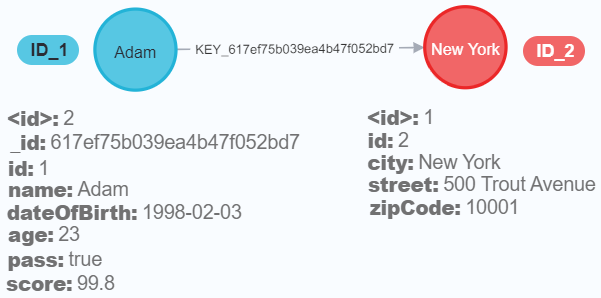
\includegraphics[width=12cm]{images/zagnieżdżenie_doc2graph.png}
\caption{Rezultat replikacji struktury z obiektem zagnieżdżonym przez Doc2graph.}
\label{fig:graf-struktura-zagnieżdżenie-doc2graph}
\end{figure}

Oba węzły wynikowe posiadają etykiety utworzone na podstawie wartości pola \texttt{id} ze struktury dokumentowej połączonego z przedrostkiem ``ID\_''. Etykieta krawędzi pomiędzy węzłami powstała przez złączenie przedrostka ``KEY\_'' i wartości identyfikatora \texttt{\_id} dokumentu studenta.

Jako że Doc2graph nie implementuje replikacji dla edycji, niemożliwe jest wykonanie edycji, która skutkowałaby replikacją - podobnie jak w przypadku struktury prostej, jedyną opcją jest usunięcie całego dokumentu lub edytowanego pola i~ponowne wstawienie zaktualizowanej zawartości. Usunięcie dokumentu z zagnieżdżeniem zakończyło się prawidłowym odwzorowaniem tej operacji w bazie grafowej i usunięciem obu węzłów.

Dla narzędzia Mongo4j stworzono odpowiedni schemat odpowiadający rozpatrywanej strukturze z zagnieżdżonym dokumentem. Dokument wstawiony za pomocą aplikacji do bazy dokumentowej przedstawia listing \ref{listing:dokument-zagnieżdżenie-mongo4j}. Odpowiadający mu graf zreplikowany w bazie Neo4j przedstawia rysunek \ref{fig:graf-struktura-zagnieżdżenie-mongo4j}. Tak jak dla poprzednich narzędzi, również w tym przypadku, w bazie grafowej powstały dwa węzły połączone krawędzią skierowaną do węzła adresu. Właściwości obu węzłów grafu poprawnie odpowiadają polom dokumentu źródłowego. Obydwa węzły posiadają właściwość \texttt{m\_id} przechowującą identyfikator odpowiadający polu \texttt{\_id} z bazy dokumentowej. Węzeł studenta otrzymał etykietę \texttt{Student}, a węzeł adresu otrzymał etykietę \texttt{Address} - odpowiadają one nazwom modeli utworzonych w oparciu o schematy. Krawędź łącząca węzły posiada etykietę stworzoną poprzez złączenie etykiet węzłów.

\captionsetup{justification=centering}
\begin{lstlisting}[style=JSON, caption={Struktura dokumentu z obiektem zagnieżdżonym wstawiona przez Mongo4j.}, label={listing:dokument-zagnieżdżenie-mongo4j}, captionpos=b]
{
  "_id" : ObjectId("617f126dc955fde8c8155164"),
  "name" : "Adam",
  "age" : 23,
  "dateOfBirth" : "1998-02-03",
  "score" : NumberDecimal("99.8"),
  "pass" : true,
    "address" : {
    "street" : "500 Trout Avenue",
    "city" : "New York",
    "zipCode" : "10001",
    "_id" : ObjectId("617f126dc955fde8c8155165")
  }, "__v" : 0
}
\end{lstlisting}

\begin{figure}[!h]
\centering
\captionsetup{justification=centering}
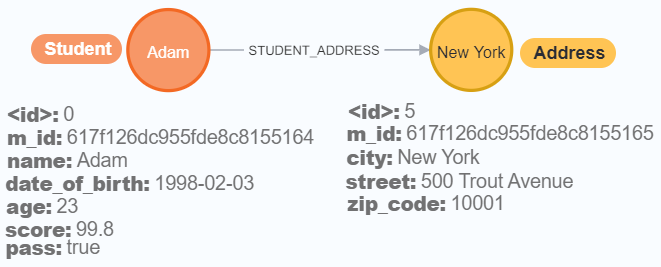
\includegraphics[width=12cm]{images/zagnieżdżenie_mongo4j.png}
\caption{Rezultat replikacji struktury z obiektem zagnieżdżonym przez Mongo4j.}
\label{fig:graf-struktura-zagnieżdżenie-mongo4j}
\end{figure}

Kolejną operacją była edycja struktury poprzez zmianę wartości pól \texttt{score} studenta i \texttt{city} adresu. W obu bazach edycja została zaaplikowana prawidłowo. Usunięcie struktury również zostało poprawnie zrealizowane w obu systemach.

\subsection{Lista elementów prostych}

Trzeci przypadek testowy sprawdza replikację dla dokumentu zawierającego listę typów prostych.
Na listingu \ref{listing:json-prosta-lista} zamieszczono rozpatrywaną strukturę. Zawiera takie same pola jak omawiana wcześniej struktura prosta oraz dodatkowe pole przechowujące listę elementów typu String. 

\begin{lstlisting}[style=JSON, caption={Struktura dokumentu z listą prostych elementów.}, label={listing:json-prosta-lista}, captionpos=b !h]
{
  "name": "Adam",
  "age": 23,
  "dateOfBirth": "1998-02-03",
  "score": 99.8,	
  "pass": true,
  "courses": ["Biology", "Chemistry", "Physics"]
}
\end{lstlisting}

\begin{figure}[bp!]
\centering
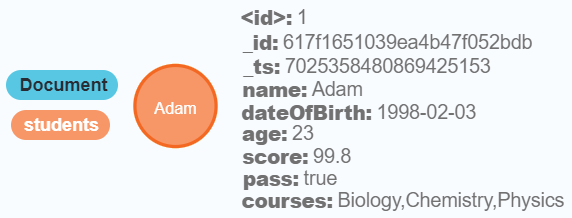
\includegraphics[width=12cm]{images/lista_prosta_neo4jdocmanager.png}
\caption{Rezultat replikacji dokumentu z listą prostych elementów przez Neo4j Doc Manager.}
\label{fig:graf-lista-prosta-neo4jdocmanager}
\end{figure}

Strukturę dodano do bazy dokumentowej przy uruchomionej replikacji narzędzia Neo4j Doc Manager i uzyskano rezultat przedstawiony na rysunku \ref{fig:graf-lista-prosta-neo4jdocmanager}. W~Neo4j utworzony został jeden węzeł, w którym lista kursów została zapisana jako kolekcja przypisana do właściwości \texttt{courses}. Węzeł otrzymał takie same etykiety, jak w poprzednich dwóch przypadkach dla tego narzędzia.

Po wstawieniu, dokument zmodyfikowano poprzez przypisanie nowej listy kursów do pola \texttt{courses} z dodatkowym wpisem. Zmiana została poprawnie zaaplikowana także w bazie grafowej. W kolejnym etapie usunięto strukturę studenta z~bazy dokumentowej, co poskutkowało poprawnym usunięciem węzła z Neo4j.   

W celu przetestowania narzędzia Doc2graph dostosowano strukturę dokumentu do postaci przedstawionej na listingu \ref{listing:json-prosta-lista-doc2graph}, poprzez dodanie pola \texttt{id}. Na skutek wstawienia dokumentu do MongoDB, w bazie grafowej uzyskano rezultat widoczny na rysunku \ref{fig:graf-lista-prosta-doc2graph}. 

\begin{figure}[h]
\begin{lstlisting}[style=JSON, caption={Struktura dokumentu z listą prostych elementów dla Doc2graph.}, label={listing:json-prosta-lista-doc2graph}, captionpos=b]
{
  "id": 1,
  "name": "Adam",
  "age": 23,
  "dateOfBirth": "1998-02-03",
  "score": 99.8,	
  "pass": true,
  "courses": ["Biology", "Chemistry", "Physics"]
}
\end{lstlisting}
\end{figure}

\begin{figure}[!h]
\centering
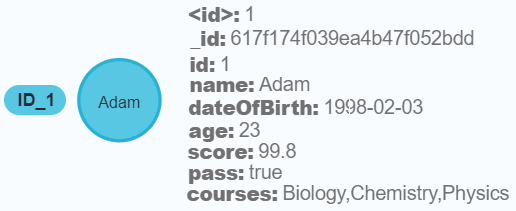
\includegraphics[width=12cm]{images/lista_prosta_doc2graph.png}
\caption{Rezultat replikacji dokumentu z listą prostych elementów przez Doc2graph.}
\label{fig:graf-lista-prosta-doc2graph}
\end{figure}

Węzeł wynikowy zawiera poprawnie odwzorowaną listę wartości typu String. Pozostałe właściwości oraz etykiety węzła powstały identycznie jak w~poprzednich przypadkach dla Doc2graph. 
Edycja listy elementów prostych z~replikacją do bazy grafowej jest niemożliwa, ponieważ Doc2graph nie replikuje operacji modyfikacji. Usunięcie dokumentu replikowane jest poprawnie.

Dla Mongo4j stworzono schemat analogicznie do poprzednich przypadków testowych. Do bazy dokumentowej wstawiony został dokument widoczny na listingu \ref{listing:dokument-lista-prosta-mongo4j}. W bazie grafowej uzyskano odwzorowanie przedstawione na rysunku \ref{fig:graf-lista-prosta-mongo4j}. W~wynikowym węźle nie pojawiła się właściwość odpowiadająca polu \texttt{courses}. 

\begin{lstlisting}[style=JSON, caption={Struktura dokumentu z listą prostych elementów wstawiona do bazy dokumentowej przez Mongo4j.}, label={listing:dokument-lista-prosta-mongo4j}, captionpos=b]
{
  "_id" : ObjectId("617f218c3fb30cacb3d81b53"),
  "name" : "Adam",
  "age" : 23,
  "dateOfBirth" : "1998-02-03",
  "score" : NumberDecimal("99.8"),
  "pass" : true,
  "courses" : ["Biology", "Chemistry", "Physics"],
  "__v" : 0
}
\end{lstlisting}

\begin{figure}[!h]
\centering
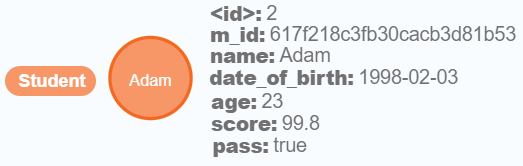
\includegraphics[width=12cm]{images/lista_prosta_mongo4j.png}
\caption{Rezultat replikacji dokumentu z listą prostych elementów przez Mongo4j.}
\label{fig:graf-lista-prosta-mongo4j}
\end{figure}

Operację wstawiania próbowano wykonać z użyciem dwóch różnych wersji schematu. Pierwsza z nich przedstawiona na listingu \ref{listing:schemat1-lista-prosta-mongo4j} skutkowała błędami i nieudanym wstawianiem danych, a druga przedstawiona na listingu \ref{listing:schemat2-lista-prosta-mongo4j} skutkowała wykonaniem replikacji bez błędów, lecz bez uwzględnienia pola \texttt{courses} w węźle wynikowym. W bazie dokumentowej lista elementów prostych wstawiana była prawidłowo niezależnie od wersji schematu.

\begin{lstlisting}[style=JSON, caption={Fragment pierwszej wersji schematu dla pola kursów.}, label={listing:schemat1-lista-prosta-mongo4j}, captionpos=b]
courses: {
  type: [String],
  neo_prop: true
}
\end{lstlisting}

\begin{lstlisting}[style=JSON, caption={Fragment drugiej wersji schematu dla pola kursów.}, label={listing:schemat2-lista-prosta-mongo4j}, captionpos=b]
courses: [{
  type: String,
  neo_prop: true
}]
\end{lstlisting}

W następnym kroku wykonano edycję pola \texttt{courses} poprzez dodanie nowej wartości. W~bazie dokumentowej zmiany zostały wprowadzone prawidłowo, natomiast w~Neo4j, gdzie pole nie istniało, nie wystąpiła żadna zmiana. Po edycji pomyślnie usunięto struktury istniejące w obu systemach.

\subsection{Lista dokumentów zagnieżdżonych}

W tym przypadku testowym weryfikowano poprawność replikacji dla dokumentu zawierającego listę dokumentów zagnieżdżonych. Rozpatrywana struktura znajduje się na listingu \ref{listing:json-lista-obiektów}. Pole \texttt{courses} przechowuje listę obiektów reprezentujących kursy - każdy kurs posiada pole nazwy \texttt{name} oraz pole długości trwania kursu \texttt{duration}.

\begin{lstlisting}[style=JSON2, caption={Struktura dokumentu z listą dokumentów zagnieżdżonych.}, label={listing:json-lista-obiektów}, captionpos=b]
{
  "name": "Adam",
  "age": 23,
  "dateOfBirth": "1998-02-03",
  "score": 99.8,	
  "pass": true,
  "courses": [
    {"name": "Biology", "duration": 3},
    {"name": "Chemistry", "duration": 1},
    {"name": "Physics", "duration": 2}
  ]
}
\end{lstlisting}

\begin{figure}[h]
\centering
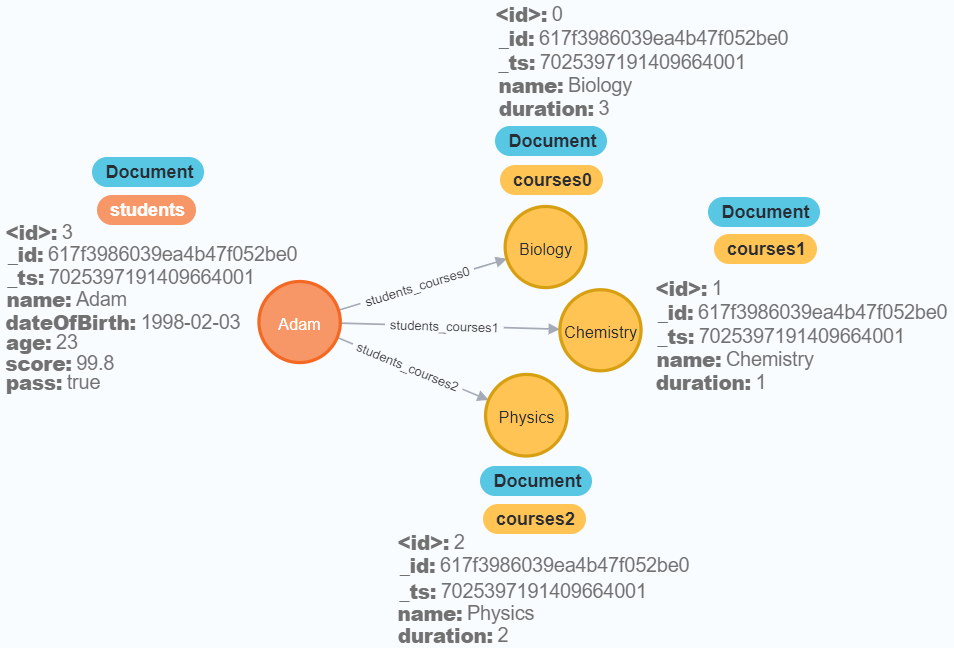
\includegraphics[width=11.4cm]{images/lista_obiektów_neo4jdocmanager.png}
\caption{Rezultat replikacji dokumentu z listą dokumentów zagnieżdżonych przez Neo4j Doc Manager.}
\label{fig:graf-lista-obiektów-neo4jdocmanager}
\end{figure}

Strukturę wstawiono do bazy dokumentowej przy załączonej replikacji za pomocą narzędzia Neo4j Doc Manager i otrzymano rezultat widoczny na rysunku \ref{fig:graf-lista-obiektów-neo4jdocmanager}. W bazie grafowej powstał węzeł studenta połączony z trzema węzłami kursów krawędziami skierowanymi do węzłów zagnieżdżonych. 
Każdy węzeł kursu posiada właściwości odpowiadające polom \texttt{name} oraz \texttt{duration}. Etykiety kursów utworzono za pomocą złączenia nazwy pola przechowującego listę kursów i wartości liczbowej oznaczającej pozycję danego kursu w liście.

Następnie wykonano operację edycji zmieniając pola dokumentów zagnieżdżonych w liście \texttt{courses}. Niestety zmiany zostały wprowadzone wyłącznie w strukturze dokumentowej. Nie udało się uzyskać odwzorowania tej operacji w bazie grafowej - implementacja Neo4j Doc Manager nie wspiera replikacji w przypadku edycji listy zagnieżdżonych obiektów. Po próbach edycji wykonano operację usuwania obiektu studenta. W wyniku tego cała struktura została usunięta z bazy dokumentowej, a w bazie grafowej pomyślnie zrealizowano odwzorowanie tej operacji. 

Na potrzeby testów narzędzia Doc2graph dostosowano strukturę dokumentu poprzez dodanie pola \texttt{id} do wszystkich dokumentów, uzyskując strukturę przedstawioną na listingu \ref{listing:json-lista-obiektów-doc2graph}. Strukturę wstawiono do bazy dokumentowej przy załączonej replikacji z użyciem narzędzia Doc2graph. Rezultat replikacji widoczny jest na rysunku \ref{fig:graf-lista-obiektów-doc2graph}. W bazie grafowej znalazły się węzły odpowiadające studentowi i trzem kursom. Właściwości węzłów poprawnie odwzorowują wszystkie pola z dokumentu źródłowego.

\begin{lstlisting}[style=JSON2, caption={Struktura dokumentu z listą dokumentów zagnieżdżonych dla Doc2graph.}, label={listing:json-lista-obiektów-doc2graph}, captionpos=b]
{
  "id": 1,
  "name": "Adam",
  "age": 23,
  "dateOfBirth": "1998-02-03",
  "score": 99.8,	
  "pass": true,
  "courses": [
    {"id": 2, "name": "Biology", "duration": 3},
    {"id": 3, "name": "Chemistry", "duration": 1},
    {"id": 4, "name": "Physics", "duration": 2}
  ]
}
\end{lstlisting}

\begin{figure}
\centering
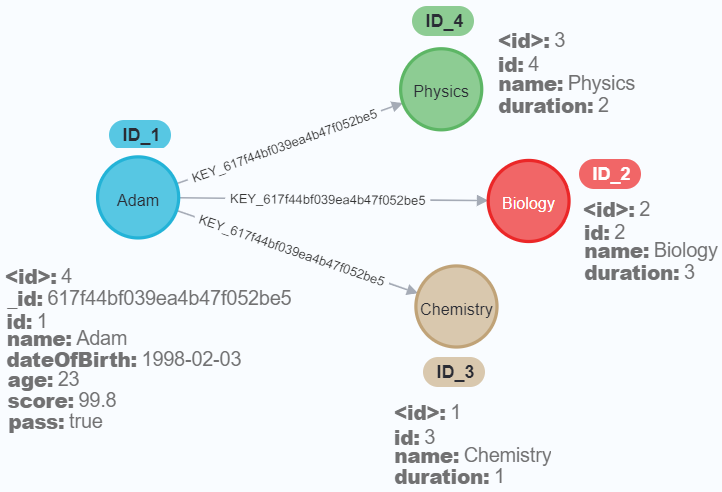
\includegraphics[width=12cm]{images/lista_obiektów_doc2graph.png}
\caption{Rezultat replikacji dokumentu z listą dokumentów zagnieżdżonych przez Doc2graph.}
\label{fig:graf-lista-obiektów-doc2graph}
\end{figure}

\vspace{0.1cm}

Każdy węzeł posiada etykietę składającą się ze złączenia przedrostka ``ID\_'' i~wartości pola \texttt{id} dokumentu źródłowego. Węzeł studenta połączony jest krawędziami z węzłami kursów, a etykiety krawędzi składają się z przedrostka ``KEY\_'' połączonego z wartością identyfikatora dokumentu, czyli pola \texttt{\_id}. Tak jak w poprzednich przypadkach dla Doc2graph, nie jest wspierana replikacja operacji edycji. Usunięcie struktury studenta w MongoDB poprawnie poskutkowało usunięciem wszystkich węzłów z bazy grafowej. 

\vspace{0.1cm}

Dla narzędzia Mongo4j stworzono odpowiedni schemat i wykonano zapis dokumentu. Dokument dodany do bazy dokumentowej widoczny jest na listingu \ref{listing:dokument-lista-obiektów-mongo4j}, a rezultat replikacji do bazy grafowej na rysunku \ref{fig:graf-lista-obiektów-mongo4j}. W bazie grafowej uzyskano graf składający się z węzła studenta i trzech węzłów kursów. Wszystkie pola proste odwzorowano w odpowiadające im właściwości. Pole \texttt{\_id} dokumentu, w węźle zapisane jest jako właściwość \texttt{m\_id}. Każdy węzeł posiada etykietę odpowiadającą nazwie modelu, dla węzła studenta jest to \texttt{Student}, a dla węzłów kursów \texttt{Course}. Krawędzie skierowane są do obiektów zagnieżdżonych z listy, a etykiety krawędzi stanowią złączenie etykiet połączonych węzłów.

\vspace{0.5cm}

\begin{lstlisting}[style=JSON, caption={Struktura dokumentu z listą dokumentów zagnieżdżonych wstawiona do bazy dokumentowej przez Mongo4j.}, label={listing:dokument-lista-obiektów-mongo4j}, captionpos=b]
{
  "_id" : ObjectId("617f31faac959e1444e5e6bf"),
  "name" : "Adam",
  "age" : 23,
  "dateOfBirth" : "1998-02-03",
  "score" : NumberDecimal("99.8"),
  "pass" : true,
  "courses" : [ 
    {
      "name" : "Biology",
      "duration" : NumberDecimal("3"),
      "_id" : ObjectId("617f31faac959e1444e5e6c0")
    }, 
    {
      "name" : "Chemistry",
      "duration" : NumberDecimal("1"),
      "_id" : ObjectId("617f31faac959e1444e5e6c1")
    }, 
    {
      "name" : "Physics",
      "duration" : NumberDecimal("2"),
      "_id" : ObjectId("617f31faac959e1444e5e6c2")
    }
  ],
  "__v" : 0
}
\end{lstlisting}

\begin{figure}
\centering
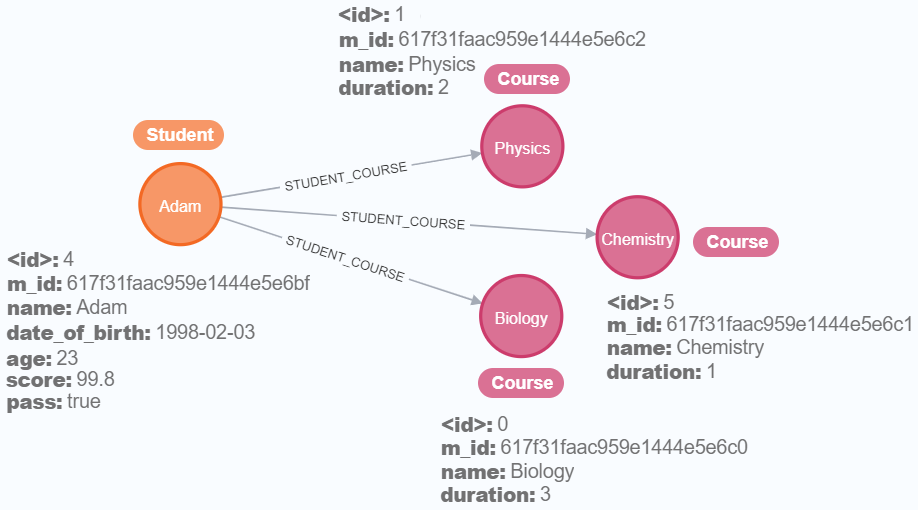
\includegraphics[width=12cm]{images/lista_obiektów_mongo4j.png}
\caption{Rezultat replikacji dokumentu z listą dokumentów zagnieżdżonych przez Mongo4j.}
\label{fig:graf-lista-obiektów-mongo4j}
\end{figure}

Po wstawieniu struktury dokonano jej edycji. W tym celu zmodyfikowano tablicę kursów oraz wartość pola przechowującego datę urodzenia. Aktualizacja w~bazie MongoDB przebiegła prawidłowo. Odwzorowanie tej operacji w bazie Neo4j również zrealizowano pomyślnie. Na końcu usunięto obiekt studenta. W wyniku tego, w bazie dokumentowej cała struktura została usunięta, a w bazie grafowej usunięto cały graf związany z danym studentem.

\subsection{Rozbudowany przykład}
\label{section:rozbudowany-przykład}

Bazując na doświadczeniu zdobytym podczas badań omawianych we wcześniejszych podsekcjach, utworzono strukturę stanowiącą rozbudowany przykład, który obejmuje wszystkie dotychczas testowane struktury. Przygotowany przypadek testowy przedstawiony jest na listingu \ref{listing:dokument-rozbudowany-przypadek-testowy}. Dla każdego narzędzia dodano dwa dokumenty zbudowane w oparciu o zaprojektowaną strukturę. W przypadku narzędzia Doc2graph w każdym obiekcie struktury dodatkowo dodano unikalne pole \texttt{id}, zgodnie z wymaganiami narzędzia.

\begin{lstlisting}[style=JSON, caption={Struktura rozbudowanego przypadku testowego.}, label={listing:dokument-rozbudowany-przypadek-testowy}, captionpos=b]
{
  "name": "Biology",
  "teacher": { 
    "firstname": "John",  
    "lastname": "Adams"
  },
  "students": [
    {
      "firstname": "Amy",
      "lastname": "Smith",
      "address": {
        "city": "New York", 
        "street": "7381 Loop St."
      },
      "marks": [5,5,5],
      "pass": true
    },
    {
      "firstname": "James",
      "lastname": "Lawrence",
      "address": {
        "city": "Los Angeles", 
        "street": "8410 Locust St."
       },
      "marks": [3.5,4,5],
      "pass": true
    }
  ]
}
\end{lstlisting}

Przy wstawianiu dokumentu odkryto, że Neo4j Doc Manager niepoprawnie obsługuje dokumenty, w których w dowolnym miejscu struktury powtarza się nazwa pola przechowującego obiekt zagnieżdżony. Na rysunku \ref{fig:graf-rozbudowana-struktura-neo4jdocmanager} przedstawiono rezultat replikacji. Widać na nim, że narzędzie dodało tylko jeden węzeł adresu połączony z obydwoma węzłami studentów. Wynika to z wewnętrznej implementacji narzędzia, w którym parsowany jest dokument i tworzona jest lista wszystkich koniecznych zapytań Cypher tworzących węzły. Gdy narzędzie napotyka konieczność stworzenia węzła o etykiecie, która została już wcześniej wykryta, poprzednie zapytanie dla tej etykiety jest nadpisywane.

\begin{figure}
\centering
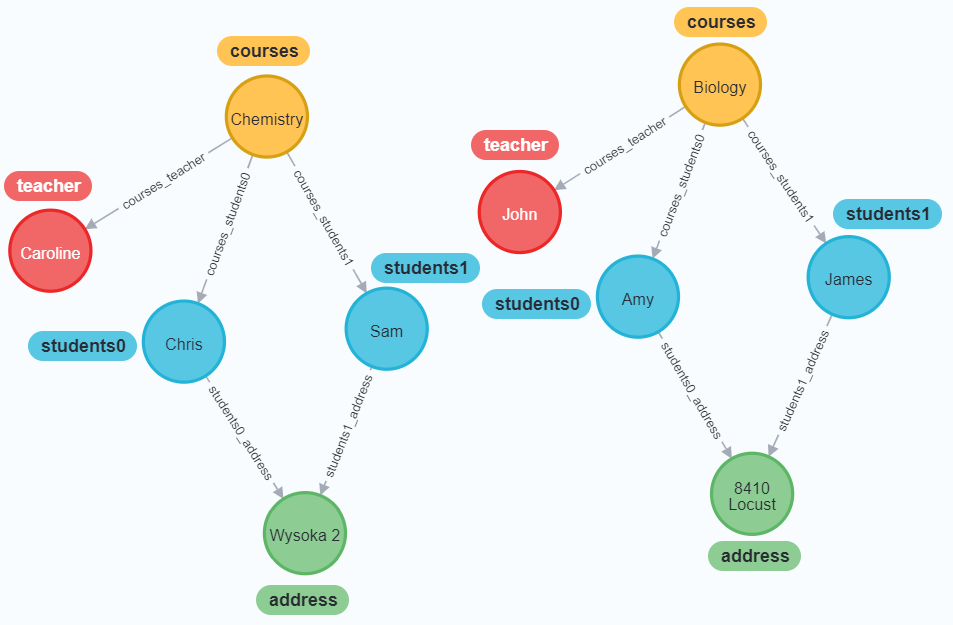
\includegraphics[width=14cm]{images/rozbudowana_struktura_neo4jdocmanager.png}
\caption{Rezultat replikacji rozbudowanych struktur przez Neo4j Doc Manager.}
\label{fig:graf-rozbudowana-struktura-neo4jdocmanager}
\end{figure}

W przeciwieństwie do poprzedniego narzędzia, Doc2graph prawidłowo przeprowadził replikację wstawiania dokumentów. Wynik replikacji zamieszczono na rysunku \ref{fig:graf-rozbudowana-struktura-doc2graph}, na którym widać, że dla dodanych dokumentów zostały utworzone dwa grafy. Każdy z nich zawiera węzeł kursu powiązany z węzłem nauczyciela i~dwoma węzłami studentów, a każdy student połączony jest z odpowiadającym mu węzłem adresu. 

\begin{figure}[!h]
\centering
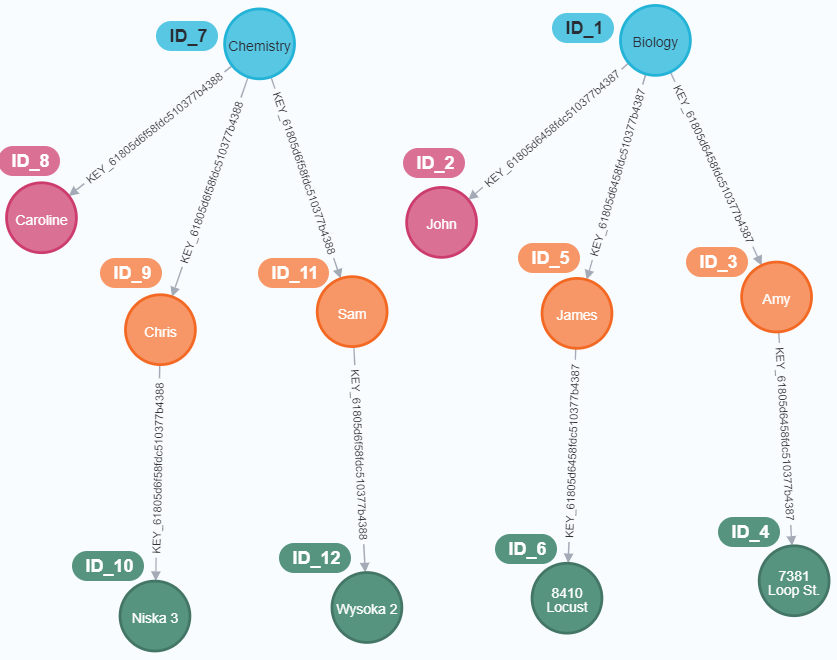
\includegraphics[width=14cm]{images/rozbudowana_struktura_doc2graph.png}
\caption{Rezultat replikacji rozbudowanych struktur przez Doc2graph.}
\label{fig:graf-rozbudowana-struktura-doc2graph}
\end{figure}

Dla narzędzia Mongo4j, podczas wstawiania dokumentu okazało się, że wielokrotne zagnieżdżenia nie są odwzorowywane w grafie. Na rysunku \ref{fig:graf-rozbudowana-struktura-mongo4j} prezentującym efekt końcowy replikacji można zauważyć, że węzły odpowiadające kursom, studentom i nauczycielom zostały dodane poprawnie ale węzły związane z~obiektami adresów zostały całkowicie pominięte, pomimo że do bazy MongoDB wstawiono kompletne struktury. W takiej sytuacji alternatywnym rozwiązaniem może być spłaszczenie struktury i odwzorowanie pól zagnieżdżonego obiektu jako właściwości węzła dokumentu przechowującego obiekt zagnieżdżony.

\begin{figure}[!h]
\centering
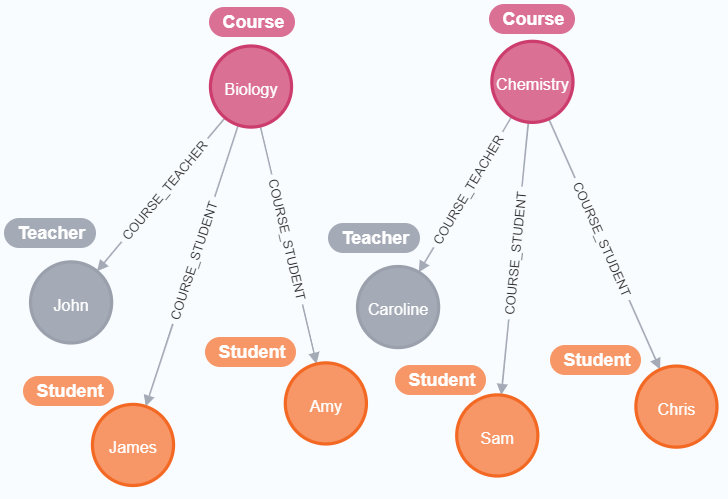
\includegraphics[width=14cm]{images/rozbudowana_struktura_mongo4j.png}
\caption{Rezultat replikacji rozbudowanych struktur przez Mongo4j.}
\label{fig:graf-rozbudowana-struktura-mongo4j}
\end{figure}

\section{Odporność na błędy} 

Analizowane narzędzia przetestowano także pod kątem stabilności i reakcji na błędy. Dla każdego z nich zasymulowano wystąpienie awarii bazy docelowej poprzez wyłączenie systemu Neo4j przed wstawieniem danych do bazy źródłowej. Dla narzędzi, których podstawą jest Mongo Connector, niedługo po zatrzymaniu bazy grafowej pojawił się błąd informujący o przekroczeniu maksymalnej ilości prób nawiązania połączenia z Neo4j, a sam Mongo Connector wyłączył się. Po wznowieniu działania bazy docelowej i ponownym uruchomieniu Mongo Connector'a replikacja została wznowiona od ostatniej poprawnie przetworzonej operacji. 

W przypadku Mongo4j, próba wstawienia danych gdy baza docelowa jest wyłączona, skutkuje błędem z informacją o nieudanym połączeniu. Mimo to, dane wstawiane są do bazy dokumentowej, a operacja dla bazy docelowej zostaje nieodwracalnie utracona. Mongo4j tylko jednokrotnie próbuje wykonać każdą operację replikacji i nie ma żadnego mechanizmu umożliwiającego odzyskanie spójności systemów po awarii. Dla Mongo4j zasymulowano także awarię bazy źródłowej, poprzez wyłączenie bazy dokumentowej, tak aby dostępna była wyłącznie baza grafowa. W~takiej sytuacji również zwracany jest błąd, jednak dane nie zostają wstawione do żadnej z baz. Brak możliwości poprawnego wznowienia pracy po awarii jest bardzo dużą wadą Mongo4j.    

Podczas wielogodzinnego i aktywnego korzystania z narzędzi, w przypadku rozwiązań opartych o Mongo Connector zaobserwowano sporadyczne problemy ze stabilnością - narzędzie przestawało przeprowadzać replikację i konieczne było jego ponowne uruchomienie. Prawdopodobnie jest to skutek problemów w implementacji samego Mongo Connector'a. Zaletą narzędzia jest to, że po ponownym uruchomieniu replikacji, wznawiana była od momentu zatrzymania, dzięki czemu zachowana jest spójność danych w obu bazach. Niestety, jeśli Mongo Connector napotka w dzienniku operacji MongoDB zmianę, której nie jest w stanie obsłużyć, to przy każdym ponownym jego uruchomieniu próbuje tę zmianę zrealizować, co skutkuje ponownymi błędami i jego zatrzymaniem. Stanowi to duży problem, bo ogranicza możliwości operowania na bazie MongoDB i wymusza na użytkowniku znajomość narzędzia replikacji. 

\section{Kompletność replikacji}

Biorąc pod uwagę wyniki badań, można ocenić jak bardzo kompletna i precyzyjna jest replikacja przeprowadzana przez analizowane narzędzia. Spośród badanych rozwiązań, tylko Neo4j Doc Manager zachował w grafie informację o nazwie kolekcji, z której pochodziły wstawione dane - pozostałe narzędzia nie przenosiły tej informacji.

Wszystkie narzędzia z wyjątkiem Mongo4j poprawnie przenosiły tablice typów prostych. W przypadku Mongo4j informacja o takiej tablicy była całkowicie tracona. Inaczej natomiast wyglądała sprawa replikacji tablicy dokumentów. Odwzorowanie tej struktury zostało zrealizowane dla wszystkich badanych narzędzi. Wynik takiego odwzorowania był identyczny jak dla replikacji dokumentów zagnieżdżonych. Niestety w większości narzędzi brakuje informacji pozwalających na rozróżnienie w bazie grafowej struktur zagnieżdżonych od obiektów wchodzących w skład tablicy. Jedynie Neo4j Doc Manager dokonał tego poprzez dodanie do etykiety węzła przyrostka w postaci liczby odpowiadającej pozycji elementu w~tablicy.

W trakcie testów zauważono, że w przypadku narzędzia Neo4j Doc Manager tracone są informacje o zagnieżdżonych obiektach, których nazwa pola powtarza się w dowolnym miejscu struktury. Doc2graph natomiast nie przenosił do grafu informacji o nazwie pola, do którego przypisany jest zagnieżdżony dokument lub tablica dokumentów.

Niestety żadne z narzędzi nie tworzy kompletnego odwzorowania utworzonej struktury dokumentowej. We wszystkich przypadkach przeniesione informacje były w mniejszym bądź większym stopniu niepełne. Bazując na grafie powstałym na skutek tak zrealizowanej replikacji, niemożliwe jest dokładne odtworzenie pierwotnej struktury z bazy źródłowej.

\section{Wnioski}

Badania wykazały, że wszystkie testowane narzędzia posiadają duże braki w~zakresie wspieranych operacji na źródłowej bazie dokumentowej. Dla przykładu, Mongo4j omija pola będące tablicą elementów typu prostego, a Doc2graph wcale nie obsługuje operacji edycji. Wszystkie tego typu problemy bardzo ograniczają przydatność narzędzi - w rozwiązaniach komercyjnych preferowane może być stworzenie nowego rozwiązania, które nie posiada takich braków.

Narzędzia oparte o Mongo Connector od dłuższego czasu nie są aktualizowane i wymagają dostosowania do pracy z nowymi wersjami baz danych. Dodatkowo, posiadają zależność do niedostępnej już publicznie wersji biblioteki py2neo. Na potrzeby badań dostosowano narzędzia Neo4j Doc Manager i Doc2graph do pracy z nowszą wersją Neo4j i aktualną wersją biblioteki py2neo. 

Narzędziem najbardziej zgodnym z przedstawionymi w pracy uniwersalnymi regułami replikacji między bazą dokumentową a grafową okazał się być Neo4j Doc Manager. Jako jedyny podczas replikacji zachował informację o kolekcji i pozwala odróżnić obiekty zagnieżdżone od tych, które wchodziły w skład tablicy. Wiele zasad działania tego narzędzia pokrywa się z opracowanym zbiorem reguł. Co prawda, wykryto błędy w implementacji, które zmniejszają poziom poprawności odwzorowania struktury w grafie ale są one na tyle proste do naprawienia, że po wprowadzeniu odpowiednich poprawek narzędzie zyskałoby pełną zgodność z~zaproponowanymi zasadami replikacji.

W kwestii wznowienia działania w sytuacji błędu lub awarii, dobrze wypadają narzędzia oparte o Mongo Connector. Umożliwiają one powtórzenie wszystkich zmian, które nie zostały zaaplikowane z powodu utraty połączenia z bazą docelową. Zapewniają kontynuację replikacji po ponownym nawiązaniu połączenia z~bazą. Znacznie gorzej wypadło narzędzie Mongo4j, które próbuje wykonać każdą operację tylko jednokrotnie, a po napotkaniu awarii nie ponawia próby realizacji operacji.

Warto zwrócić uwagę, że przeprowadzone testy badały poprawność replikacji zmian, a nie skupiały się na szybkości wprowadzania zmian w bazie docelowej. Mierzenie czasu replikacji poszczególnych operacji byłoby bardzo skomplikowane, a ponadto w zdecydowanej większości typowych przypadków użycia replikacji wysoka szybkość przenoszenia zmian nie jest krytyczna. Dużo bardziej istotna jest dokładność odwzorowania zmian i zapewnienie spójności danych pomiędzy systemami.

\chapter{Podsumowanie}

Celem niniejszej pracy było przeprowadzenie analizy możliwości replikacji danych między bazą dokumentową a grafową. Przybliżono charakterystykę tych systemów oraz szczegółowo przedstawiono uniwersalny zestaw reguł replikacji danych pomiędzy bazą dokumentową a grafową. Do dokładnej analizy wybrano trzy narzędzia wspierające replikację: Mongo4j, Neo4j Doc Manager i Doc2graph. Narzędzia poddano testom pod kątem poprawności replikacji i zgodności z zaprezentowanymi wcześniej regułami replikacji. 

Wprowadzenie replikacji do dowolnego systemu informatycznego wiążę się z~dodatkową pracą i kosztami. Konieczna jest konfiguracja mechanizmów replikacji oraz stałe monitorowanie i utrzymywanie replik i serwerów, na których są przetrzymywane. Zachowanie spójności w systemach korzystających z replikacji jest nietrywialne i może wpływać na wydajność systemu. Biorąc to pod uwagę, przed zastosowaniem replikacji należy rozważyć potrzeby systemu i ocenić, czy zalety takiego rozwiązania przewyższają jego wady.

Wybór narzędzi wspierających replikację między bazą dokumentową a grafową jest bardzo ograniczony. Większość dostępnych narzędzi nie jest już wspierana ani aktualizowana. Jedyną aktywnie utrzymywaną opcją jest Mongo4j, które jednak oparte jest na bibliotece Mongoose i wymaga predefiniowanych schematów danych, przez co jest mało uniwersalne.

Wykorzystanie nowych mechanizmów dostępnych w bazach danych może pozwolić na implementację bardziej nowoczesnych i wydajnych rozwiązań replikacji. Strumienie zmian (Change Streams) dostępne w MongoDB mogą dostarczać informacji o wszystkich wykonywanych operacjach na poziomie dowolnej bazy lub pojedynczej kolekcji. Ponadto pozwalają odtworzyć wszystkie zdarzenia od wybranego momentu w czasie. Dla replikacji danych z bazy grafowej do dokumentowej, dostępny jest analogiczny mechanizm Neo4j Streams, który pozwala wysyłać informacje o zmianach wykonanych w bazie Neo4j.

Przygotowany w ramach pracy uniwersalny zestaw reguł replikacji pomiędzy bazą dokumentową a grafową prezentuje sposób konwersji dowolnie złożonych dokumentów do struktury grafowej, z zachowaniem wszystkich informacji przechowywanych w bazie dokumentowej. Zasady replikacji można stosować w stosunku do dowolnych implementacji systemów grafowych i dokumentów, nie tylko przy wykorzystaniu omawianych w pracy baz MongoDB i Neo4j. Dodatkowo, dzięki zachowaniu kompletnych informacji podczas konwersji, możliwe jest potencjalne przywrócenie danych źródłowych. Wymagałoby to przygotowania reguł dedykowanych procesowi replikacji danych z bazy grafowej do dokumentowej. Konieczna byłaby również implementacja narzędzia realizującego ten proces, np. wykorzystując mechanizm Neo4j Streams.

W celu pełnego wykorzystania przedstawionych reguł replikacji między bazą dokumentową a grafową, konieczne byłoby zaimplementowanie nowego rozwiązania. Przy tworzeniu takiego narzędzia wskazane byłoby uwzględnienie replikacji aktualnego stanu danych w bazie źródłowej, a następnie realizacja dynamicznej replikacji przyrostowej. Dodatkowo korzystne może być udostępnienie możliwości monitorowania procesu, z uwzględnieniem mierzenia czasu trwania operacji wykonywanych na bazie docelowej i źródłowej. Takie rozwiązanie byłoby bardziej kompleksowe od dostępnych obecnie narzędzi. 


%%%%%%%%%%%%%%%%%%%%%%%%%%%%%%%%%%%%%%%%%%
\backmatter
\pagenumbering{Roman}
\stepcounter{stronyPozaNumeracja}
\setcounter{page}{\value{stronyPozaNumeracja}}

\pagestyle{tylkoNumeryStron}

%%%%%%%%%%% bibliografia %%%%%%%%%%%%
\bibliographystyle{plplain}
\bibliography{bibliografia}
\addcontentsline{toc}{chapter}{Bibliografia}
%%%%%%%%%  DODATKI %%%%%%%%%%%%%%%%%%% 

\begin{appendices} 


% \chapter*{Dokumentacja techniczna}
% \addcontentsline{toc}{chapter}{Dokumentacja techniczna}

\chapter*{Spis skrótów i symboli}
\addcontentsline{toc}{chapter}{Spis skrótów i symboli}

\begin{itemize}
\item[ACID] Atomicity, Consistency, Isolation, Durability - Atomowość, Spójność, Izolacja, Trwałość
\item[API] Application Programming Interface - interfejs programowania aplikacji
\item[AWS] Amazon Web Services - platforma usług w chmurze
\item[CMS] Content Mangagement System - system zarządzania treścią
\item[PyPI] Python Package Index - repozytorium pakietów dla języka Python
\item[RSZBD] Relacyjny System Zarządzania Bazą Danych (ang. \ang{Relational Database Management System})
\item[SQL] Structured Query Language - strukturalny język zapytań
\item[SZBD] System Zarządzania Bazą Danych (ang. \ang{Database Management System})
\end{itemize}
 

\chapter*{Zawartość dołączonej płyty}
\addcontentsline{toc}{chapter}{Zawartość dołączonej płyty}

Do pracy dołączona jest płyta CD z~następującą zawartością:
\begin{itemize}
\item praca magisterska w~formacie \texttt{pdf},
\item źródła \LaTeX owe (katalog ``Praca magisterska - źródła''), 
\item poprawione pliki źródłowe dla narzędzia Neo4j Doc Manager (katalog ``Tools\textbackslash Neo4jDocManager''), 
\item poprawione pliki źródłowe dla narzędzia Doc2graph (katalog ``Tools\textbackslash Doc2graph''), 
\item źródła aplikacji używającej Mongo4j (katalog ``Tools\textbackslash Mongo4j''), 
\item pliki konfiguracyjne dla narzędzi Neo4j Doc Manager, Doc2graph i Mongo4j wraz z bazami MongoDB i Neo4j (katalog ``Docker''). 
\end{itemize}

Zawartość płyty dostępna jest również w repozytorium GitHub pod adresem:
\url{https://github.com/oladyr/MasterThesis}

\vspace{0.3cm}

Przygotowane obrazy badanych narzędzi dostępne są w repozytoriach Docker Hub pod następującymi adresami:
\begin{itemize}
\item \url{https://hub.docker.com/r/oladyr/neo4j-doc-manager},
\item \url{https://hub.docker.com/r/oladyr/doc2graph},
\item \url{https://hub.docker.com/r/oladyr/mongo4j}.
\end{itemize}

\makeatletter
\def\@tocrmarg{2.55em plus 3em}
\makeatother
\listoffigures

\addcontentsline{toc}{chapter}{Spis rysunków}
% \listoftables
% \addcontentsline{toc}{chapter}{Spis tabel}

\renewcommand*{\lstlistlistingname}{Spis listingów}
\lstlistoflistings
	
\end{appendices}


\end{document}


%% Finis coronat opus.
